

\part{Coding Agent Training with Scalable Synthetic Data}
\label{part:scalability}


\start{Overview of Part~\ref{part:scalability}}
This part comprises two chapters organized around a single theme: \emph{by reducing the complexity of constructing training data in appropriate ways, we could potentially improve scalability while preserving effectiveness}.
 
Chapter~\ref{chap:cmtrans} illustrates this idea through a code translation task. A key bottleneck of the scale of training data is the difficulty of obtaining parallel data pairs (i.e., functionally equivalent code written in different programming languages).
To address this, we show that constructing comparable code pairs (i.e., code snippets with similar functionality) is substantially easier, and that training on such pairs remains effective. Experiments further demonstrate that combining comparable and parallel data significantly outperforms training on parallel data alone.

Chapter~\ref{chap:repost} applies the same principle to training coding agents. Here, the primary bottleneck is constructing the training environment: typical workflows require installing an entire repository (on average 26.5 external packages), which demands substantial effort from both humans and agents. We mitigate this challenge by bypassing repository installation via sandbox testing, which greatly simplifies environment construction (by installing only 2.1 packages per instance). Importantly, the resulting training examples remain effective because the agent can still access the full repository when completing the task.

% Chapter~\ref{chap:effective-analysis} outlines a proposed work aimed at empirically answering the question: “what makes a training trajectory effective” for coding agents. We first show that even successful trajectories on the same set of instances can vary widely in effectiveness. We then propose to identify the characteristics that distinguish trajectories generated by different teacher models.
% Finally, we propose to improve trajectory effectiveness by injecting beneficial characteristics into training trajectories.




\chapter{Constructing Scalable Code Translation Training Data with Comparable Corpora and Multiple References \textcolor{aquablue}{(\textit{completed})}}
\label{chap:cmtrans}


\newcommand{\hlours}[1]{%
  \begingroup
  \sethlcolor{#1}%
  \hl{ CMTrans }%
  \endgroup
}

\begin{figure}[t]
    \centering
    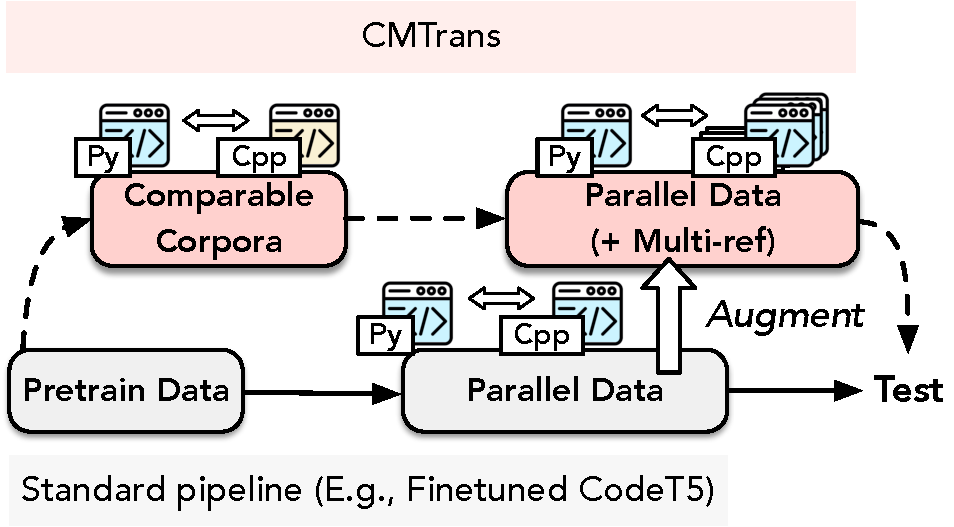
\includegraphics[width=0.5\linewidth]{CMTrans_figs/diagram_intro_v2.pdf}
    \caption{The standard pipeline for code translation (colored in light grey) and the CMTrans pipeline (colored in pink). The comparable corpora are both naturally occurring and model generated. We generate multiple references by \cmtransours.
    }
    \label{fig:cmtrans_diagram_intro}
\end{figure}

\begin{figure}[t]
    \centering
    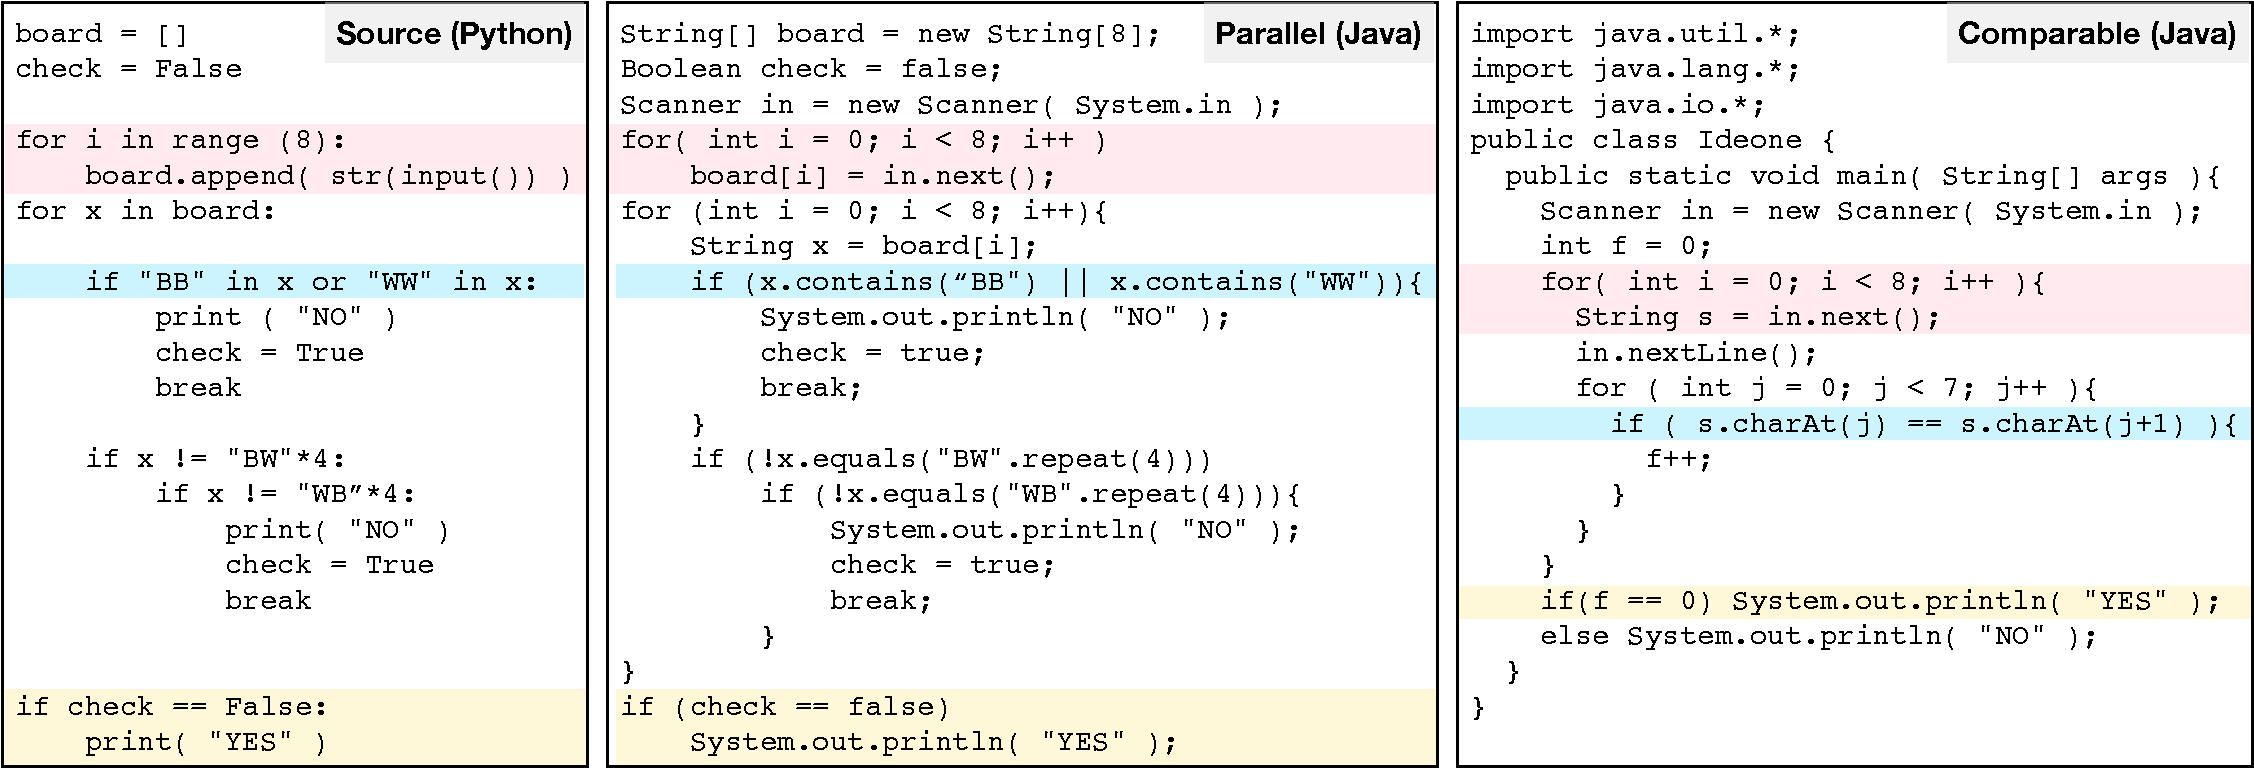
\includegraphics[width=\linewidth]{CMTrans_figs/examples_intro.pdf}
    \caption{An example of parallel and comparable data. Parallel examples are line-by-line aligned. Programs in a comparable example may have different algorithms and structures (e.g., global code vs. class in this case), but may still contain lines that can be matched, as highlighted in pink, blue, and yellow.}
    \label{fig:cmtrans_example_intro}
\end{figure}


\begin{figure}[t]
  \centering

  \begin{subfigure}[t]{0.4\linewidth}
    \centering
    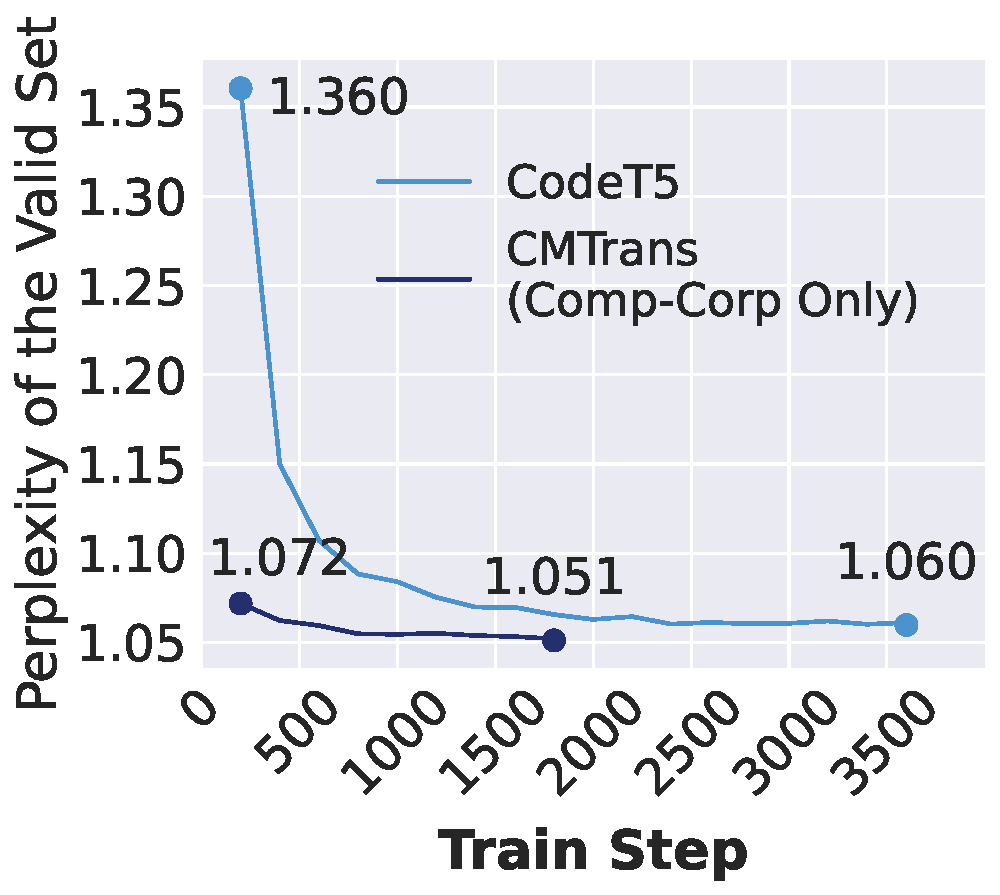
\includegraphics[width=\linewidth]{CMTrans_figs/ppl_java2python.pdf}
    \caption{Java-to-Python}
    \label{fig:cmtrans_ppl1}
  \end{subfigure}
  % \hfill%
  \begin{subfigure}[t]{0.4\linewidth}
    \centering
    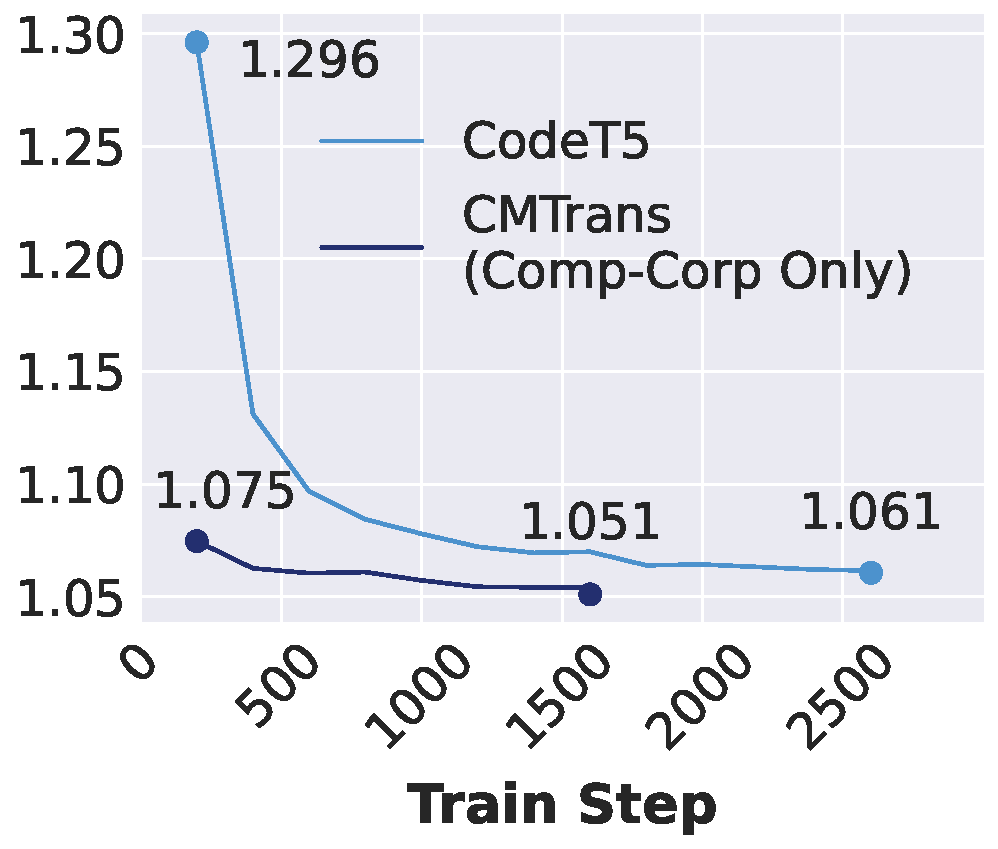
\includegraphics[width=\linewidth]{CMTrans_figs/ppl_python2java.pdf}
    \caption{Python-to-Java}
    \label{fig:cmtrans_ppl2}
  \end{subfigure}

  \caption{Perplexity of validation set during finetuning.}
  \label{fig:cmtrans_ppl}
\end{figure}


\section{Introduction}
In this chapter, we show a successful case of constructing scalable and effective training data for code translation.

% [motivate code translation]
Code translation is a special type of machine translation that translates between programming languages.
It is widely applied in software engineering to migrate a codebase into another programming language.
Recent code translation models typically follow the pretrain-finetune pipeline.
As shown in \autoref{fig:cmtrans_diagram_intro}, in pretraining, with denoising objectives such as masked span or identifier prediction \cite{plbart,codet5,transcoder}, the model learns to produce sequences in both languages.
When finetuned on parallel data \cite{avatar}, which are program pairs in the source and target language that are aligned line-by-line, the model learns functional equivalence: identifying programs with the same functionality,
either in the same language or between languages.
We show an example of parallel data in \autoref{fig:cmtrans_example_intro}.

One major challenge of code translation is that parallel data is typically limited. For instance, the TransCoder dataset \cite{transcoder} only contains 466 Python-C++ pairs. Constructing parallel data requires substantial human effort and cannot be easily scaled. 
With limited fine-tuning examples, it is difficult for a model to learn functional equivalence across programming styles and domains.

To mitigate the data scarcity issue, we pose three questions: \textbf{
(1) What does the model need to learn to perform code translation? 
(2) Does everything need to be learned from parallel data?
(3) If parallel data is still necessary, how to obtain parallel data in an efficient way?}

We answer the first question: what the model needs to learn, by comparing the model before and after finetuning. We observe that (1) the model learns to generate fluent code in the target language. As shown in \autoref{fig:cmtrans_ppl}, with the source language as input, before finetuning, the model continues to generate code in the source language, and the ground truth translation in the target language has a high perplexity.
(2) The model learns the functionality equivalence between the source and target languages. Namely, it learns the implementation of the same functionality in both languages. 

% [present the solution: comparable corpora of different types]
As for the second question, we show that both (1) and (2) can be learned from \emph{comparable corpora} to some extent, a term we borrow from natural language translation, where it refers to texts on similar topics in different languages \cite{NMTComparableCorpora,low_resource_comp_corpora}.
Here, we use it to refer to programs with similar functionality in different languages \cite{avatar,xcodeeval}.
As shown in \autoref{fig:cmtrans_example_intro}, although the programs paired in a comparable example may have different algorithms and structures (e.g., global code vs.\ class functions), they are likely to have similar constructs and may even have some lines that can be matched.

% [in this paper, the CC part]
In this paper, we \emph{study what the model learns from comparable corpora} by building three types of comparable examples:
(1) \emph{Naturally existing}, where we leverage independently-written solutions of the same coding problem;
(2) \emph{Generated}, where we collect programs with docstrings in one language and apply a code generation model to generate programs in another language; and
(3) \emph{Retrieved}, where we either retrieve a program's k nearest neighbors (KNN) or simply choose a random program in another language.
Among them, (1) contains cleaner examples, which are guaranteed to be bug-free. (3) covers programs from a larger variety of sources, providing more diverse training signals.

Since comparable corpora only contain program pairs with similar functionality, parallel data is still necessary to translate the precise functionality across different programming languages. 
As an answer to the third question, we notice that the majority of finetuning data only have one reference translation (e.g., 82.5\% in AVATAR, \citealt{avatar}).
However, code with different surface forms may have the same functionality (e.g., the interchange between \texttt{for loops} and \texttt{while loops}).
This makes it possible to augment the dataset by adding multiple reference translations with the same functionality, which reduces overfitting to a single translation and boosts the model to fully capture code semantics.

As a result, in this paper, we \emph{generate multiple translation references} for the finetuning data.
Specifically, after training on comparable corpora, we finetune a model on the original parallel data, generate multiple translations for each example, and use automatically generated test cases to filter out incorrect translations.
By training on different functionally equivalent programs, we reduce overfitting to a single output and improve the modeling of the target language.


% [results and analysis]
Combining the two techniques, we name our full approach \cmtransours, a code \textbf{Trans}lation model trained with \textbf{C}omparable corpora and \textbf{M}ultiple references.
Extensive experiments show that \cmtransours significantly improves CodeT5 \cite{codet5}, which is initialized from the same pretrained checkpoint, for an average of 7.5\% Computational Accuracy (CA@1) over translation between 6 language pairs.
\cmtransours also significantly outperforms the state-of-the-art method in 5 out of 6 language pairs, while reaching parity on the other one.

Analyses of our two techniques suggest that:
(1) All three types of comparable corpora (including random program pairs) improve the syntax accuracy and perplexity of the translation outputs and lead to better final performance.
(2) Both naturally existing and generated comparable corpora help the model generate constructs that match the input. The combination of them gives the largest performance gain.
(3) By training with multiple references, the model generates more unique correct translations within a certain budget, which indicates that better functional equivalence of the target language is learned.


% \section{Related Work}
% \start{Code Translation}
% Previous work has tackled the problem of translating code written in one programming language to another. 
% \citet{Karaivanov2014PhraseBasedST}, \citet{Nguyen2013LexicalSM,Nguyen2015DivideandConquerAF}, \citet{Phan2017StatisticalMO,Oda2015LearningTG} applied statistical machine translation techniques to code translation, while \citet{TreetotreeNN} introduced a tree-to-tree neural translation approach. 
% Further improvements were achieved by pre-trained language models of code such as CodeBERT \cite{codebert}, PLBART \cite{plbart}, and CodeT5 \cite{codet5}. 
% However, the above approaches require finetuning on parallel data, which is often scarce. 

% \start{Data Scarcity in Code Translation}
% To tackle the data scarcity issue, TransCoder \cite{transcoder} uses back translation for unsupervised code translation.
% DOBF \cite{dobf}, TransCoder-ST \cite{transcoderST}, and S\&G \cite{SandG} respectively improve TransCoder with de-obfuscation pre-training, self-training, and pairing up the model with a generation and a summarization model.
% However, the best-performing approach, TransCoder-ST, is only able to generate parallel data for standalone functions where the model can already generate a correct solution within a limited budget.
% In contrast, the comparable corpora we use to train \cmtransours include code with arbitrary structure and content.
% \cmtransours also has much better efficiency, as self-training requires running a much larger number of test cases than generating multiple references.
% MultiPL-E \cite{multiple} also automatically generates test cases, but retries until the output passes all test cases. We do not directly compare to it since it requires multiple rounds of translation.

% \start{Data Augmentation for Natural Language Translation}
% The lack of parallel training data is a fundamental problem in the field of translation, which has led the NLP community to develop several data augmentation techniques in response. 
% \textit{Comparable Corpora}, as defined by \citet{first_comp_corpora}, ``are texts that, while not parallel in the strict sense, are somewhat related and convey overlapping information''. 
% \citet{methods_collect_comp_corpora} and \citet{harvesting_comp_corpora} present methods for collecting comparable corpora to study when and how to use them. 
% \citet{handle_with_care_comp_corpora} and \citet{NMTComparableCorpora} identify information balance, alignment, and length differences between source and target as key factors affecting translation quality. 
% In this work, we extend the study of comparable corpora to code translation. 
% We show that code translation can benefit from multiple types of comparable corpora even if there is already high-quality parallel data. 
% We also provide analyses on why comparable corpora are beneficial.

% Another data augmentation strategy is using multiple translation references. 
% \citet{truly_exploring_multi_ref} and \citet{simulated_multi_ref} found that using multiple references can be beneficial in low-resource settings.
% An advantage of working with code is that test cases can be used to filter model-generated translated references to ensure functional equivalence to the source, which we exploit in \cmtransours.









\section{Methodology}
In this section, we introduce our data augmentation method that trains the model first on comparable corpora, which are either naturally existing, generated, or retrieved (\S\ref{sec:comparable}) and then on parallel data with additional references generated by \cmtransours (\S\ref{sec:multiref}).

\begin{figure}[t]
    \centering
    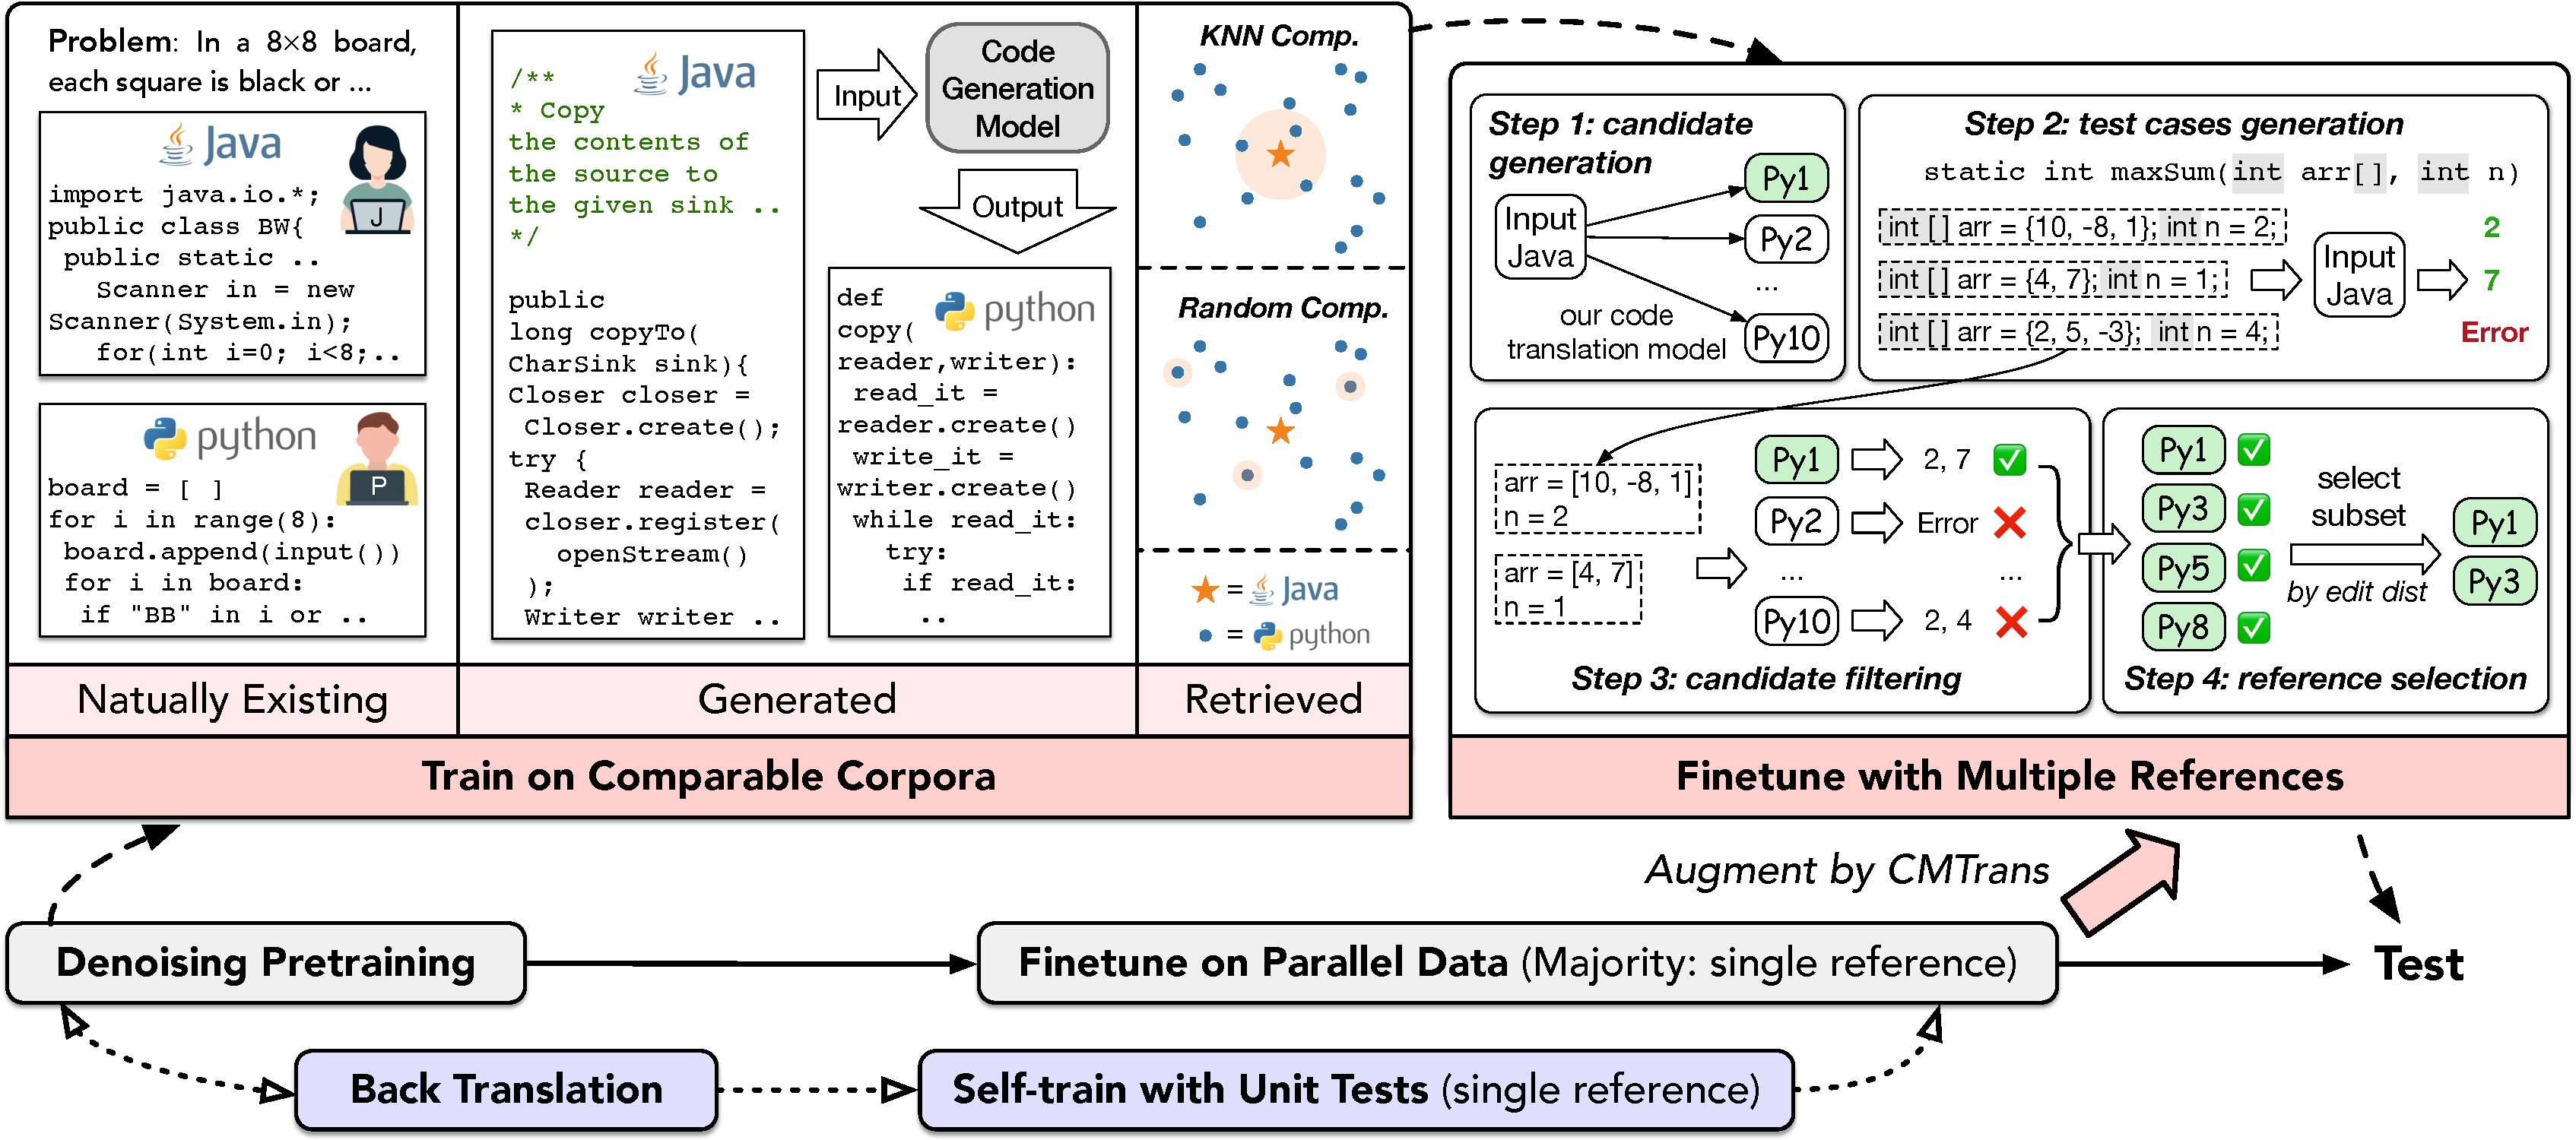
\includegraphics[width=\linewidth]{CMTrans_figs/method_v2.pdf}
    \upv
    \caption{An example of \cmtransours for Java-to-Python translation. We compare the pipeline of \cmtransours (\textit{red}) to the standard pipeline (\textit{grey}) of code translation (e.g., finetuned CodeT5, \citealt{codet5}) and the self-supervision-and-fine-tuning method (\textit{purple}) of TransCoder-ST (\citealt{transcoderST}).}
    \label{fig:cmtrans_method}
    \downv
\end{figure}

\subsection{Problem Formulation}
We formulate code translation as a sequence-to-sequence (Seq2Seq) generation problem following existing work \cite{codexglue,avatar,transcoder}.
The input is the code in the source language $S = \{s_1, s_2, ..., s_n \}$, which is a sequence of tokens.
We apply a model to translate the input code into the target language $T = \mathcal{M}_{\theta}(S) = \{t_1, t_2, ..., t_m \}$, where the model $\mathcal{M}_{\theta}$ is typically finetuned for code translation. 
Alternatively, the model may generate $k$ candidate outputs for each input: $\mathcal{M}_{\theta}(S,k) = \mathbb{T} = \{ T^{(1)}, T^{(2)}, ..., T^{(k)} \}$. 

\subsection{Training on Comparable Corpora}
\label{sec:comparable}

As shown in \autoref{fig:cmtrans_method}, we study three types of comparable corpora: naturally existing, generated, and retrieved ones. Here we introduce how we build each type of comparable examples and train \cmtransours on them.

\start{Naturally Existing Comparable Examples}
We make use of comparable corpora collected from programming contests by existing datasets \cite{avatar,xcodeeval,codenet}, which mainly consist of solutions to the same contest problems written in different languages.
These comparable examples are typically confined to specific domains such as dynamic programming or graph theory.


\start{Generated Comparable Examples}
To cover programs in more diverse domains, we present a method that automatically generates comparable examples using natural-language-to-code generation models.

Specifically, we leverage a monolingual corpus of functions with natural language documentation (i.e., docstrings) to describe their functionality.
In the experiments, we use GitHub functions with docstrings extracted by CodeSearchNet \cite{codesearchnet}.
For each function $S_c$ in the corpus, we feed the natural language documentation to a code generation model finetuned in the other language, which is trained to generate a program based on the given natural language description.
Similarly to code translation, the code generation model can generate multiple candidate outputs $\{ T_c^{(1)}, T_c^{(2)}, ..., T_c^{(k)} \}$.
We then select the one with the highest probability, which is paired up with the extracted program as a comparable example.


\start{Retrieved Comparable Examples}
To study the effect of the quality of comparable corpora, we further build \textbf{KNN Comparable Corpora}.
We compute the embedding of all the programs in the source and target language in the dataset using a finetuned code retrieval model~\cite{codesearchnet}.
For each program $S$ in the source language with embedding $emb(S)$, we retrieve its k nearest neighbors in the target language by the cosine similarity between their embeddings: $sim(S,T) = \langle emb(S), emb(T) \rangle$.

Finally, we build \textbf{Random Comparable Corpora} by pairing random programs in the source and target language.
In principle, such program pairs do not contain any information on functional equivalence and allow us to better understand whether comparable corpora can improve the modeling of the target language and hence improve the translation quality.



\start{Model Training}
After constructing a corpus of comparable examples $\mathcal{D}_c = \{(S_c, T_c)\}$, we input the program in the source language $S_c$ into \cmtransours $\mathcal{M}_{\theta}$ and maximize the log-likelihood of its corresponding program in the target language $T_c = \{t_{c,1}, t_{c,2}, ..., t_{c,m} \}$:
\begin{align}
\begin{split}
&\mathcal{L}_{M T}(\mathcal{D}_c) = \sum_{(S_c, T_c) \in \mathcal{D}_c} P_{\theta}(T_c | S_c) \\
&P_{\theta}(T_c | S_c) = -\sum_i \log \left(P_{\theta}\left(t_{c,i} | S_c, t_{c,1} \ldots t_{c,i-1} \right)\right)
\end{split}
\label{eq:mtloss}
\end{align}

Here $\theta$ is the parameter of $\mathcal{M}_{\theta}$, which is initialized from an encoder-decoder model pretrained on code \cite{codet5}.
After training the model on the corpus comparable examples $\mathcal{D}_c$ till convergence, we finetune it on the dataset of parallel examples $\mathcal{D}_p$, where the loss $\mathcal{L}_{M T}(\mathcal{D}_p)$ is computed by \autoref{eq:mtloss} as well.

By maximizing the probability of the target $T_c$, the model will learn to generate fluent code in the target language.
Furthermore, in general, programs in a comparable example often exhibit the same types of constructs.
In the examples in \autoref{fig:cmtrans_example_intro}, to check whether a board is valid, no matter what algorithm is used, the program will always need a loop to read the board and use if statements for the validity check.
As a result, in principle, the model can also learn to generate the same types of constructs as the input program $S_c$, which is beneficial for generating accurate translations.


\subsection{Finetuning with Multiple References}
\label{sec:multiref}
In addition to comparable corpora, we also provide \cmtransours with more diverse training signals by finetuning with multiple references. 
By providing the model with programs with the same functionality, we encourage the model to learn a better representation space for the target language and hence benefit the translation.

Since the majority of source programs only have one reference in existing datasets of parallel examples \cite{avatar}, we apply a series of steps to generate additional references, which are illustrated in \autoref{fig:cmtrans_method}.
The first step is to finetune a model with the original parallel data, and then use the finetuned model to generate multiple translation candidates $\{ T_c^{(1)}, T_c^{(2)}, ..., T_c^{(k)} \}$ for each source program in the parallel data.

In the second and third steps, similar to TransCoder-ST \cite{transcoderST}, we leverage automatically generated unit tests to filter out candidates with different behaviors as the source program.
Specifically, we extract the input arguments of the source programs, randomly produce a set of test inputs based on the argument types, and feed the test inputs to the source program.
We filter out test inputs that cause compilation or runtime errors.
Finally, we feed the remaining test inputs to each candidate and only keep the ones that have exactly the same output as the source program.

Notice that some of the translations may only have small differences (e.g., \texttt{i++} vs. \texttt{i+=1}). To obtain a diverse subset of references, we select the most distinct $k$ translations for each source program by their string edit distance.
These $k$ translations are added as additional references to the finetuning set.




\begin{table}[t]
\centering
\resizebox{\textwidth}{!}{
\begin{tabular}{lcccc|c}
\toprule
\multirow{2}{*}{\bf Dataset $\rightarrow$}
& \multicolumn{3}{c}{\textbf{Train (Comparable)}} & \textbf{Train (Parallel)} & \textbf{Test} \\ 
\cmidrule(lr){2-4}  \cmidrule(lr){5-5} \cmidrule(lr){6-6}
& \textbf{Gen-comp} & \textbf{XCodeEval} & \textbf{AVATAR-comp} 
& \textbf{AVATAR-para} & \textbf{TransCoder-test} \\
\midrule
\bf \# C++ $\leftrightarrow$ Java & 4,053* & 3,414 & -- & 3,226* & 482 C-to-J, 467 J-to-C \\
\bf \# C++ $\leftrightarrow$ Python & 4,053* & 4,376 & -- & 3,226* & 464 C-to-P, 467 P-to-C \\
\bf \# Java $\leftrightarrow$ Python & 22,181* & -- & 5,937 & 3,391 & 464 J-to-P, 482 P-to-J \\ 
\bf Source 
& \begin{tabular}[c]{@{}c@{}}
Github (Java $\leftrightarrow$ Python) \\
AIZU, AtCoder (Others)
\end{tabular}
& Codeforces 
& \begin{tabular}[c]{@{}c@{}} 
AtCoder, Codeforces, ProjectEuler, \\ 
CodeJam, GeeksforGeeks, LeetCode, 
\end{tabular} 
& GeeksforGeeks 
& GeeksforGeeks \\
\bottomrule
\end{tabular}
}
\caption{Number of problems per dataset. ``Gen-comp'' is the comparable corpora dataset we generate. C-to-J, C-to-P, ... denote the test examples of C++-to-Java, C++-to-Python translation, etc. * denotes data we build.}
\label{tab:cmtrans_dataset}
\end{table}







\section{Results}

\begin{table}[t]
\centering
\resizebox{0.8\textwidth}{!}{
\begin{tabular}{lccccccccc}
\toprule
\multirow{2}{*}{\bf Model $\downarrow$}
& \multicolumn{3}{c}{\bf Java-to-Python} 
& \multicolumn{3}{c}{\bf Python-to-Java} 
& \multicolumn{3}{c}{\bf Avg of 6 Pairs} 
\\
% \midrule
\cmidrule(lr){2-4}  \cmidrule(lr){5-7} \cmidrule(lr){8-10}
% \bf Model $\downarrow$
& \bf BLEU & \bf CB & \bf CA@1 
& \bf BLEU & \bf CB & \bf CA@1 
& \bf BLEU & \bf CB & \bf CA@1 \\
\midrule
TransCoder \cite{transcoder} & 72.4 & 67.9 & 49.1 & 65.4 & 70.7 & 35.7 
& 72.0 & 75.0 & 51.7 \\
DOBF \cite{dobf} & 72.2 & 67.5 & 52.2 & 67.7 & 71.2 & 44.4 
& --- & --- & --- \\
TransCoder-ST \cite{transcoderST} & 73.1 & 68.7 & 68.5 & 70.0 & 71.9 & 58.1 
& 71.3 & 74.9 & 66.3 \\
\midrule
CodeBERT \cite{codebert} & 52.0 & 48.9 & 10.4 & 45.4 & 45.0 & 4.2 
& --- & --- & --- \\
CodeT5 \cite{codet5} & 79.4 & 72.5 & 61.0 & 79.0 & 75.9 & 52.7 
& \underline{83.6} & 80.0 & 62.6 \\
PLBART \cite{plbart} & \underline{79.9} & \underline{73.2} & 68.9 & 80.5 & 76.8 & 57.5 
& --- & --- & --- \\
TransCoder-ST-ft \cite{transcoderST} & 79.3 & 72.9 & \underline{69.4} & \underline{81.4} & \underline{78.4} & \underline{62.0} 
& 81.8 & \underline{80.2} & \underline{67.6} \\
\midrule
\cmtransours & \bf 80.1 & \bf 74.2 & \bf 73.5 & \bf 84.3 & \bf 82.1 & \bf 66.0 
& \bf 84.9 & \bf 82.0 & \bf 70.1 \\ 
\bottomrule
\end{tabular}
}
\caption{Java-Python translation results on TransCoder-test. We copy the results of all the baselines reported by \citet{avatar}. 
CB and CA@1 stand for CodeBLEU and Computational Accuracy. 
We highlight the \textbf{best} results under each metric with Bold and underline the \underline{second-best} results.}
\label{tab:cmtrans_main}
\end{table}

\begin{table}[t]
\centering
\resizebox{\textwidth}{!}{
\begin{tabular}{lcccccccccccc}
\toprule
\multirow{2}{*}{\bf Model $\downarrow$}
% \midrule
& \multicolumn{3}{c}{\bf C++-to-Java} 
& \multicolumn{3}{c}{\bf C++-to-Python}
& \multicolumn{3}{c}{\bf Java-to-C++} 
& \multicolumn{3}{c}{\bf Python-to-C++} \\
% \midrule
\cmidrule(lr){2-4}  \cmidrule(lr){5-7} \cmidrule(lr){8-10} \cmidrule(lr){11-13}
& \bf BLEU & \bf CB & \bf CA@1 
& \bf BLEU & \bf CB & \bf CA@1 
& \bf BLEU & \bf CB & \bf CA@1 
& \bf BLEU & \bf CB & \bf CA@1 \\
\midrule
TransCoder \cite{transcoder} & 84.0 & 86.7 & 65.1 & 75.2 & 73.4 & 47.1 & 83.6 & 85.4 & 79.8 & 51.6 & 65.7 & 32.6 \\
TransCoder-ST \cite{transcoderST} & 78.8 & 85.2 & 68.0 & 73.1 & 73.0 & 61.3 & 76.7 & 83.7 & \bf 84.6 & 55.8 & 67.1 & 56.7 \\
\midrule
CodeT5 \cite{codet5} & \underline{90.9} & 90.0 & 65.1 & \underline{82.9} & \underline{75.4} & 56.5 & 89.1 & \bf 88.5 & 81.6 & \underline{79.8} & \underline{77.9} & 58.5 \\
TransCoder-ST-ft \cite{transcoderST} & 88.7 & \underline{90.1} & \underline{68.3} & 75.4 & 74.3 & \underline{62.5} & \underline{89.3} & 87.8 & \bf 84.6 & 76.7 & 77.6 & \underline{59.1} \\
\midrule
\cmtransours & \bf 91.6 & \bf 90.5 & \bf 71.4 & \bf 83.7 & \bf 77.2 & \bf 64.2 & \bf 89.7 & \underline{88.4} & \underline{84.4} & \bf 82.0 & \bf 79.3 & \bf 61.2 \\
\bottomrule
\end{tabular}
}
\caption{Java-C++ and Python-C++ translation results on TransCoder-test. The CA@1 results of TransCoder and TransCoder-ST are copied from the TransCoder-ST paper. We evaluate BLEU and CodeBLEU using their released checkpoints. We finetune and evaluate CodeT5 and TransCoder-ST-ft on our own.}
\label{tab:cmtrans_cpp}
\end{table}


In this section, we conduct experiments to answer four
research questions: 
(\textbf{RQ1}) How do \cmtransours and its ablations perform compared against state-of-the-art approaches for code translation?
(\textbf{RQ2}) What can the model learn from comparable corpora?
(\textbf{RQ3}) What can the model learn from multiple references? 
(\textbf{RQ4}) How is \cmtransours affected by the size of comparable corpora and the number of references?

\subsection{Experimental Setup}
\label{sec:setup}
We initialize \cmtransours from the pretrained checkpoint of CodeT5 \cite{codet5}, an encoder-decoder model pretrained on code files from varied languages with denoising objectives.

\start{Datasets}
We list the dataset statistics in \autoref{tab:cmtrans_dataset}.
All the methods are evaluated on the TransCoder-test dataset~\cite{transcoder}.
We train our method on xCodeEval \cite{xcodeeval}, a comparable corpora dataset, and AVATAR \cite{avatar}, which contain both comparable corpora and parallel functions (denoted as AVATAR-comp and AVATAR-para, respectively).
All the supervised baseline methods are finetuned on AVATAR-para before evaluation.

Since AVATAR-para does not contain C++ functions, we add a parallel C++ function for each training example in AVATAR-para. Specifically, we generate 50 C++ translations for each Java function by TransCoder-ST, TransCoder, and finetuned CodeT5 and filter the translations with unit tests.

\start{Construction of Comparable Corpora}
We conduct the study on different types of comparable corpora (\CC) on Java $\leftrightarrow$ Python translation.
We use AVATAR-comp\footnote{There are two versions of AVATAR-comp with slight differences. We use the first version because most of our experiments were finished before the second version was released.} as the naturally existing \CC.
KNN and random \CC are also retrieved from AVATAR-comp.
To build the dataset of generated \CC (denoted as Gen-Comp), we generate from functions with docstrings in the CodeSearchNet~\cite{codesearchnet} dataset.

We train \cmtransours first on the best combination of comparable corpora, which is natural and generated \CC, and then finetuned on AVATAR-para.
For language pairs other than Java $\leftrightarrow$ Python, we use xCodeEval as naturally existing \CC and generate \CC from CodeNet~\cite{codenet}. 
% More details can be found in Appendix~\ref{sec:implementation}.


\start{Evaluation metrics}
Our primary metric is the Computational Accuracy (CA@k), which evaluates whether at least 1 out of k translation candidates generates the same outputs as the reference for all the given test inputs.
Following previous work \cite{avatar}, we report \textbf{CA@1} results and also report \textbf{BLEU}, which computes the overlap between candidate and reference translations \cite{BLEU}, and \textbf{CodeBLEU}: the weighted average of token level match, syntax level match, and Dataflow match \cite{codebleu}.
% Appendix \ref{sec:implementation} contains more details about the implementation and baselines.


\subsection{Main results}
\autoref{tab:cmtrans_main} and \autoref{tab:cmtrans_cpp} show the code translation results on TransCoder-test.

\cmtransours substantially outperforms CodeT5, which is initialized from the same pretrained checkpoint and finetuned with the original parallel data, by an average improvement of 7.5\% CA@1.
\cmtransours also significantly outperforms the state-of-the-art methods, TransCoder-ST-ft, on 5 out of 6 language pairs, and reaches parity on Java-to-C++ translation.
Note that TransCoder-ST-ft generates test cases for 103,488 functions and executes these test cases over 4 iterations of training. 
In comparison, \cmtransours only generates test cases for 3,391 functions and executes the test cases once, resulting in better efficiency.

Our results show that the advantage of \cmtransours is larger on translations between Java and Python. The reason may be that the parallel data we generate for translations involving C++ are only verified by automatically generated test cases, which might not cover all the boundary cases and could introduce noise to the finetuning set.
Following previous work~\cite{transcoderST,avatar}, we report the results of one checkpoint. 
% We also conduct the t-test in Appendix~\ref{sec:ttest}, which indicates that \cmtransours significantly outperforms the best baseline over CA@1 with p-value $<$ 0.01 for 4 out of 6 language pairs and with p-value $<$ 0.05 for one language pair.

\subsection{Performance Analysis}
\start{Ablation studies}
\autoref{tab:cmtrans_ablation} presents the ablations of our approach. 
We first study the effectiveness of each type of comparable corpora and some combinations of them. All the ``+ \CC'' ablations denote training CodeT5 on comparable corpora and then finetuneing on AVATAR-para.
We also ablate ``+ Multi-Ref'', which is finetuned on multiple references directly after pretraining.
The results show that both Multi-Ref and the best \CC provide a large performance gain and stacking them (the full \cmtransours) has the best performance.

As for the effectiveness of different \CC, we can see that code translation can benefit from all these types of \CC. The combination of Natural and generated \CC has the best performance. The reason might be both \CC have relatively high data quality and further adding the other two \CC in training introduces noise to the model and hinders the learning of functional equivalence.

Notice that with the same finetuning set, \textit{\CC\ Only} still outperforms TransCoder-ST-ft, which indicates that compared to self-training, training on comparable corpora has not only better efficiency but better effectiveness.
We hypothesize that the reason may be that the comparable corpora contain more diverse structures and contents. This provides more diverse training signals to the model and hence improves the generalization.

\begin{table}[t]
\centering
\resizebox{0.6\linewidth}{!}{
\begin{tabular}{lcc}
\toprule
% \midrule
\bf Model $\downarrow$ & \bf J-to-P CA@1 & \bf P-to-J CA@1 \\
\midrule
CodeT5 & 61.0 & 52.0 \\
+ Random \CC & 64.7 & 54.6 \\
+ KNN \CC & 63.8 & 55.4 \\
+ Generated \CC & 64.0 & 63.1 \\
+ Natural \CC & 68.8 & 62.9 \\ 
\midrule
+ All \CC & 62.5 & 55.4 \\
+ Natural \& Generated & 70.0 & 64.1 \\ 
+ Multi-Ref & 68.1 & 61.6 \\ 
\cmtransours & \bf 73.5 & \bf 66.0 \\ 
\bottomrule
\end{tabular}
}
\caption{Ablation studies of \cmtransours. We report CA@1 results. J-to-P and P-to-J stand for Java-to-Python and Python-to-Java results. We put the experiments on each type of comparable corpora in an individual block.}
\label{tab:cmtrans_ablation}
\end{table}



\start{Translation with Limited Parallel Data}
To analyze how well \cmtransours tackles the data scarcity challenge, we compare the performance of CodeT5 and \cmtransours when finetuned on parallel data with different sizes.
For simplicity, we use \cmtransours (\CC Only) to denote the ``CodeT5 + Natural \& Generated'' ablation 
and use \cmtransours (Multi-Ref\ Only) to denote ``CodeT5 + Multi-Ref''.

As shown in \autoref{fig:cmtrans_size}, the relative gains of \cmtransours as well as our ablations are more pronounced when the parallel data is more limited. 
For example, when there are only 100 parallel examples for Java-to-Python translation, CodeT5 obtains 6.5 CA@1 while \cmtransours, (\CC Only), and (Multi-Ref\ Only) obtain 43.1, 39.7, and 26.9 CA@1, respectively. 
This demonstrates the effectiveness of our two data augmentation techniques to tackle data scarcity.

\begin{figure}[t]
    \centering
    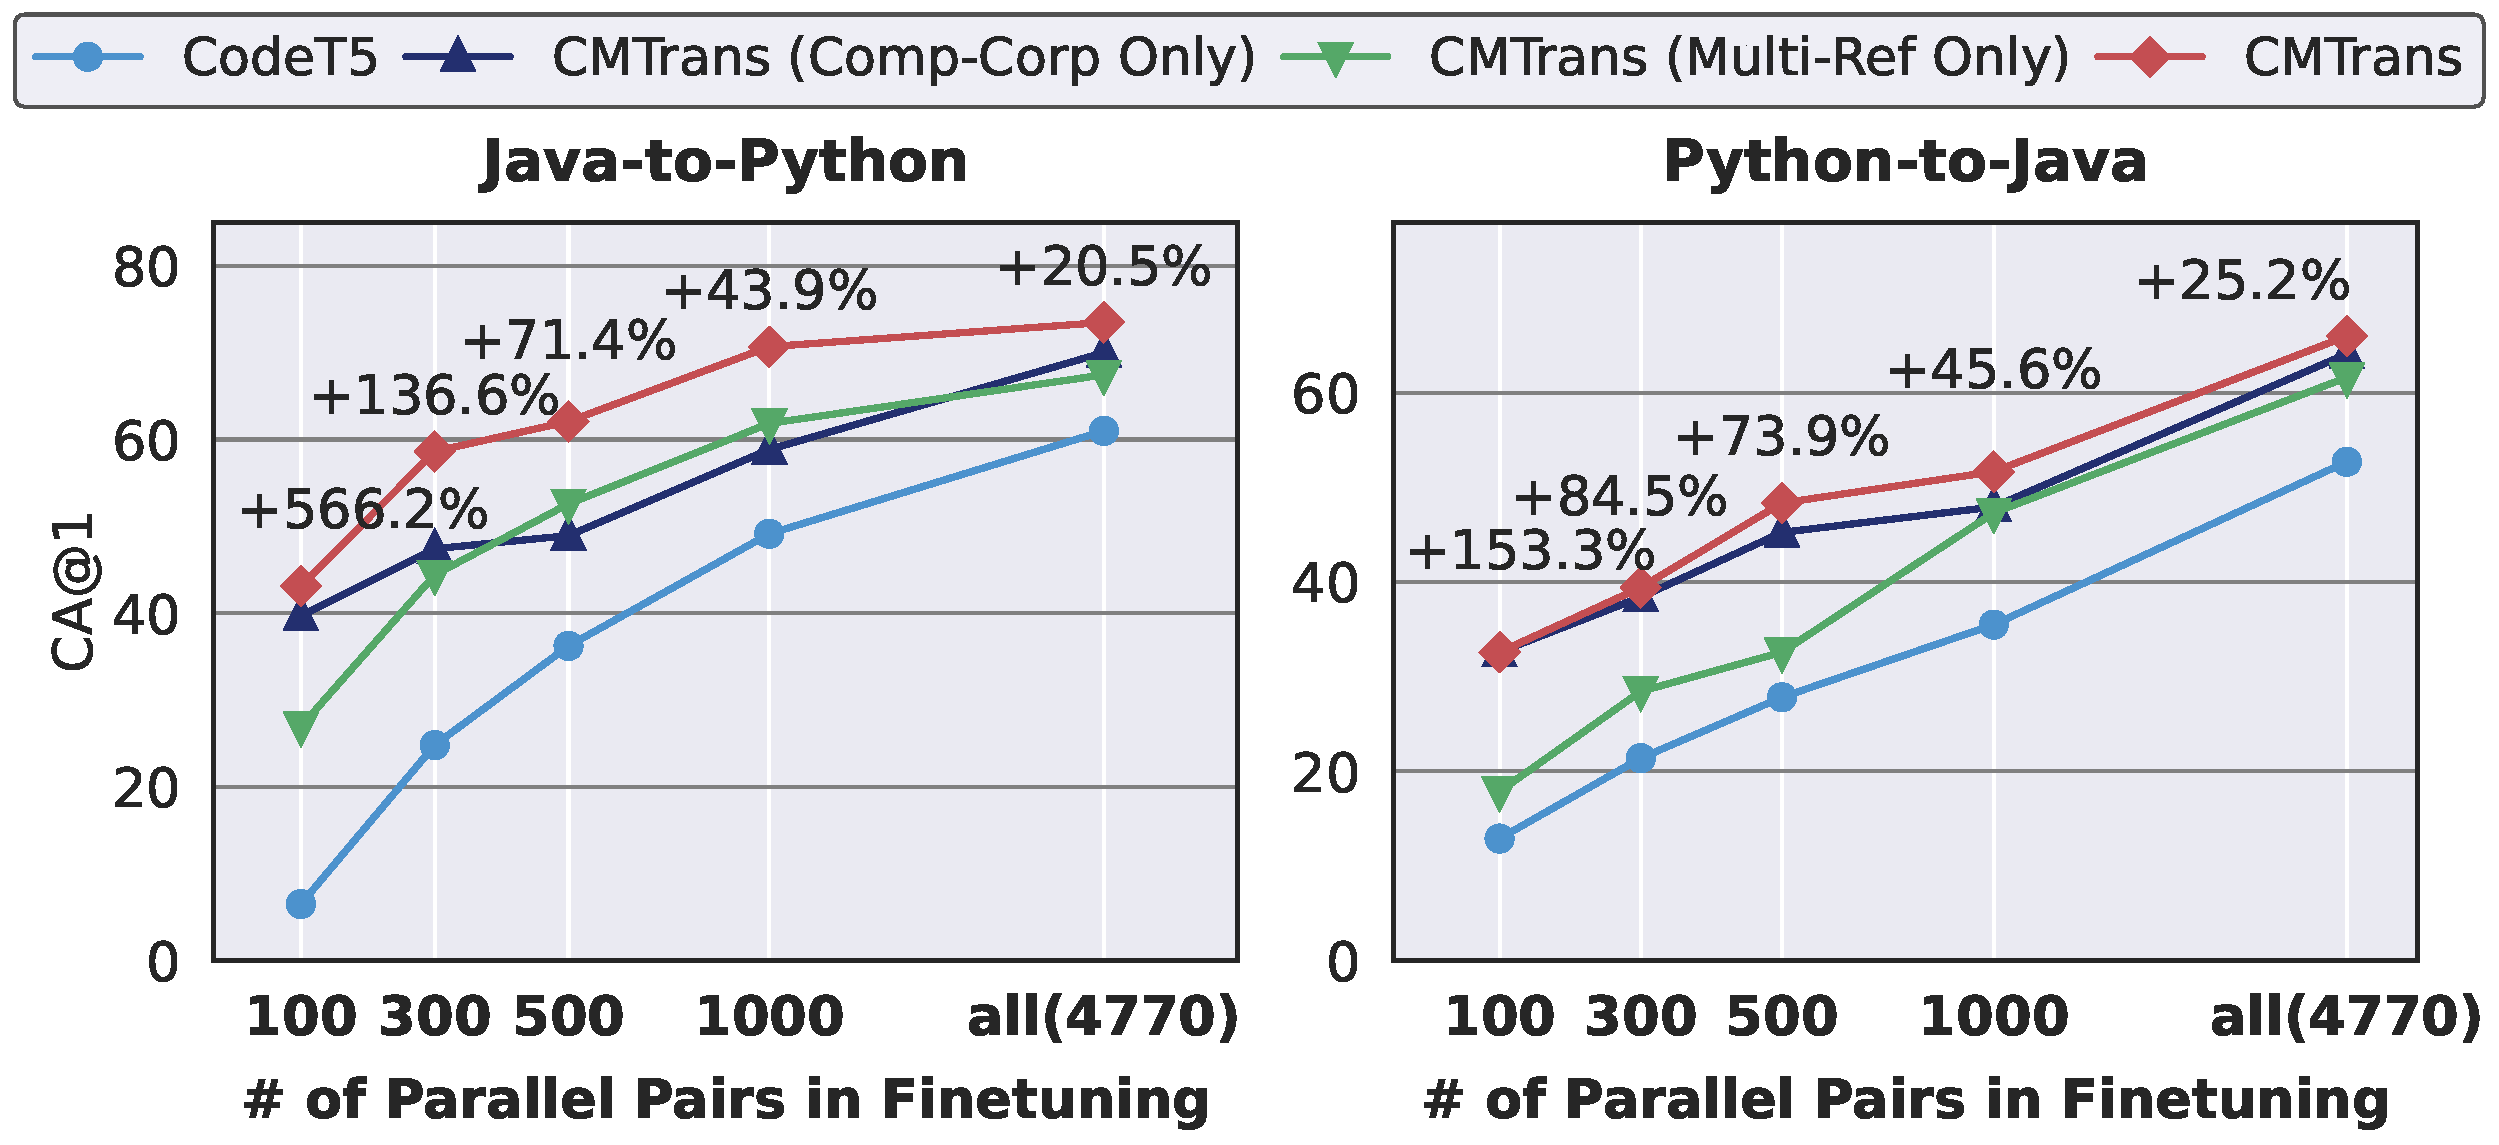
\includegraphics[width=0.7\linewidth]{CMTrans_figs/size_analysis_fig.pdf}
    \caption{Translation results with different amount of parallel data. We mark the relative gain of \cmtransours over CodeT5.}
    \label{fig:cmtrans_size}
\end{figure}

\begin{table}[t]
\centering
\resizebox{\linewidth}{!}{
\begin{tabular}{lccccccccc|ccccccccc}
\toprule
\multirow{3}{*}{\bf Model $\downarrow$}
& \multicolumn{9}{c}{\bf Java-to-Python} 
& \multicolumn{9}{c}{\bf Python-to-Java} \\
\cmidrule(lr){2-10} \cmidrule(lr){11-19} 
& \multicolumn{3}{c}{\bf LOOP} 
& \multicolumn{3}{c}{\bf IF} & \multicolumn{3}{c}{\bf ELSE IF} 
& \multicolumn{3}{c}{\bf LOOP} 
& \multicolumn{3}{c}{\bf IF} & \multicolumn{3}{c}{\bf ELSE IF} \\
\cmidrule(lr){2-4}  \cmidrule(lr){5-7} \cmidrule(lr){8-10}
\cmidrule(lr){11-13}  \cmidrule(lr){14-16} \cmidrule(lr){17-19}
& P & R & F1 & P & R & F1 & P & R & F1 
& P & R & F1 & P & R & F1 & P & R & F1 \\
 \midrule
CodeT5 (No finetune) & 100.0 & 28.5 & 44.4 & 99.1 & 35.4 & 52.2 & 0.0 & 0.0 & 0.0 &
100.0 & 14.6 & 25.5 & 100.0 & 36.6 & 53.6 & 0.0 & 0.0 & 0.0 \\
+ KNN \CC & 89.4 & 94.6 & 91.9 & 82.1 & 64.3 & 72.1 & 41.6 & 57.6 & 48.3 & 
87.9 & 98.9 & 93.1 & 90.2 & 50.9 & 65.1 & 30.5 & 16.4 & 21.3 \\
+ Generated \CC & 99.9 & 98.9 & \bf 99.4 & 99.0 & 93.2 & \bf 96.0 & 84.6 & 79.2 & \bf 81.8 & 98.3 & 96.7 & \bf 97.5 & 98.7 & 94.8 & \bf 96.7 & 83.3 & 86.4 & \bf 84.8 \\
+ Natural \CC & 95.8 & 85.4 & 90.3 & 91.2 & 73.9 & 81.6 & 50.0 & 49.6 & 49.8 & 87.4 & 98.9 & 92.8 & 88.2 & 80.4 & 84.1 & 57.8 & 33.6 & 42.5 \\
\bottomrule
\end{tabular}
}
\caption{The overlap between the types of constructs in the translation outputs and the ground truth translations. }
\label{tab:cmtrans_construct}
\end{table}


\begin{table}[t]
\centering
\resizebox{0.6\linewidth}{!}{
\begin{tabular}{lcc}
\toprule
\bf Model $\downarrow$ & \bf J-to-P SA& \bf P-to-J SA \\
\toprule
No finetuning on parallel pairs \\
\midrule
CodeT5 \cite{codet5} & 1.1 & 1.7 \\
+ Random \CC & 20.0 & 41.3 \\
+ KNN \CC & 22.0 & \bf 56.4 \\
+ Generated \CC & \bf 41.4 & 43.2 \\
+ Natural \CC & 34.1 & 54.6 \\
\toprule
With finetuning on parallel pairs \\
\midrule
CodeT5 \cite{codet5} & 95.3 & 69.7 \\
+ Random \CC & 96.3 & 69.7 \\
+ KNN \CC & 96.3 & 71.0 \\
+ Generated \CC & \bf 97.6 & 71.2 \\
+ Natural \CC & 97.4 & \bf 76.4 \\
\bottomrule
\end{tabular}
}
\caption{Syntax Accuracy (SA) on TransCoder-test before finetuning, which evaluates whether the program can be compiled without syntax errors.}
\label{tab:cmtrans_EA}
\end{table}



\subsection{Influence of Comparable Corpora}
To answer \textbf{RQ2}, we hypothesize that training on comparable corpora allows the model to produce fluent code in the target language while using similar constructs as the input.


\start{Fluency of outputs}
To validate our hypothesis, we compare the perplexity of the reference translations (in the target language) during finetuning, which reflects the fluency of outputs.
As shown in \autoref{fig:cmtrans_ppl}, after training on comparable corpora, the perplexity is substantially reduced before finetuning. It also converges to a lower value after finetuning on parallel data.

Similarly, \autoref{tab:cmtrans_EA} shows that in most scenarios, training on comparable corpora leads to fewer syntax errors both before and after finetuning, which means the programs \cmtransours generates not only have a high token-level overlap with the reference translations but are also syntactically correct.
The reason might be comparable corpora (including the random \CC) train the model to maximize the probability of a complete program in the target language, improving its language modeling ability.



\start{Generation of matching constructs}
We observe that programs in a comparable pair typically contain similar constructs (e.g., in AVATAR-comp, for 83.41\% of Java programs with if statements, the corresponding Python programs also contain if statements).
To assess whether \cmtransours also learns to generate the correct types of constructs, for each type of construct, we consider whether the reference translation has this type of construct as the ground truth and whether the translation output has it as the predictions. Then we compute the accuracy, recall, and F1 scores.

As shown in \autoref{tab:cmtrans_construct}, after training on KNN, generated, and natural \CC, the F1 score is highly improved.
The generated \CC has the highest F1 scores. The reason might be we input both the documentation and the program to the generation model, so the generated program follows the same algorithm as the input program, which results in a larger percentage of comparable examples that share the same types of constructs.


\begin{figure}[t]
    \centering % <-- added
\begin{subfigure}{0.4\linewidth}
  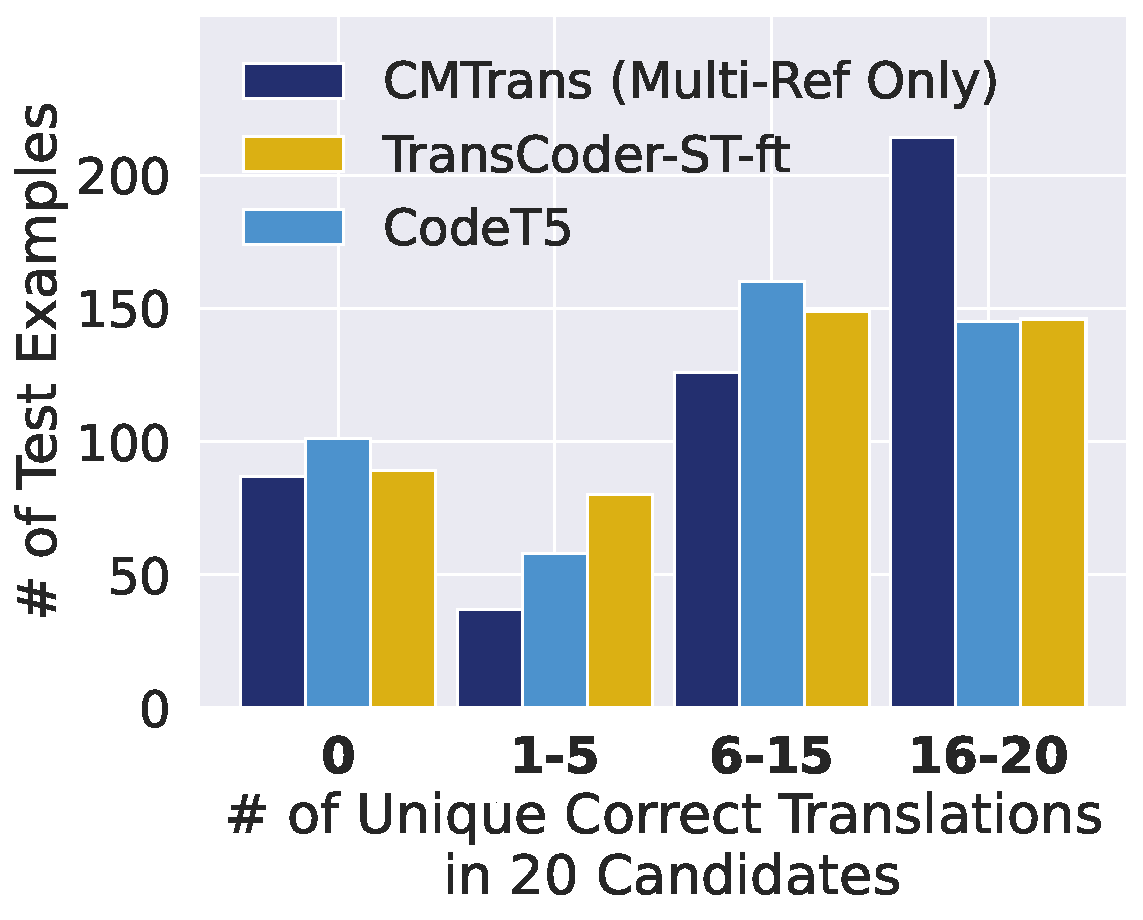
\includegraphics[width=\linewidth]{CMTrans_figs/unique_java2python.pdf}
  \caption{Java-to-Python}
  \label{fig:cmtrans_uni1}
\end{subfigure}\hfil % <-- added
\begin{subfigure}{0.4\linewidth}
  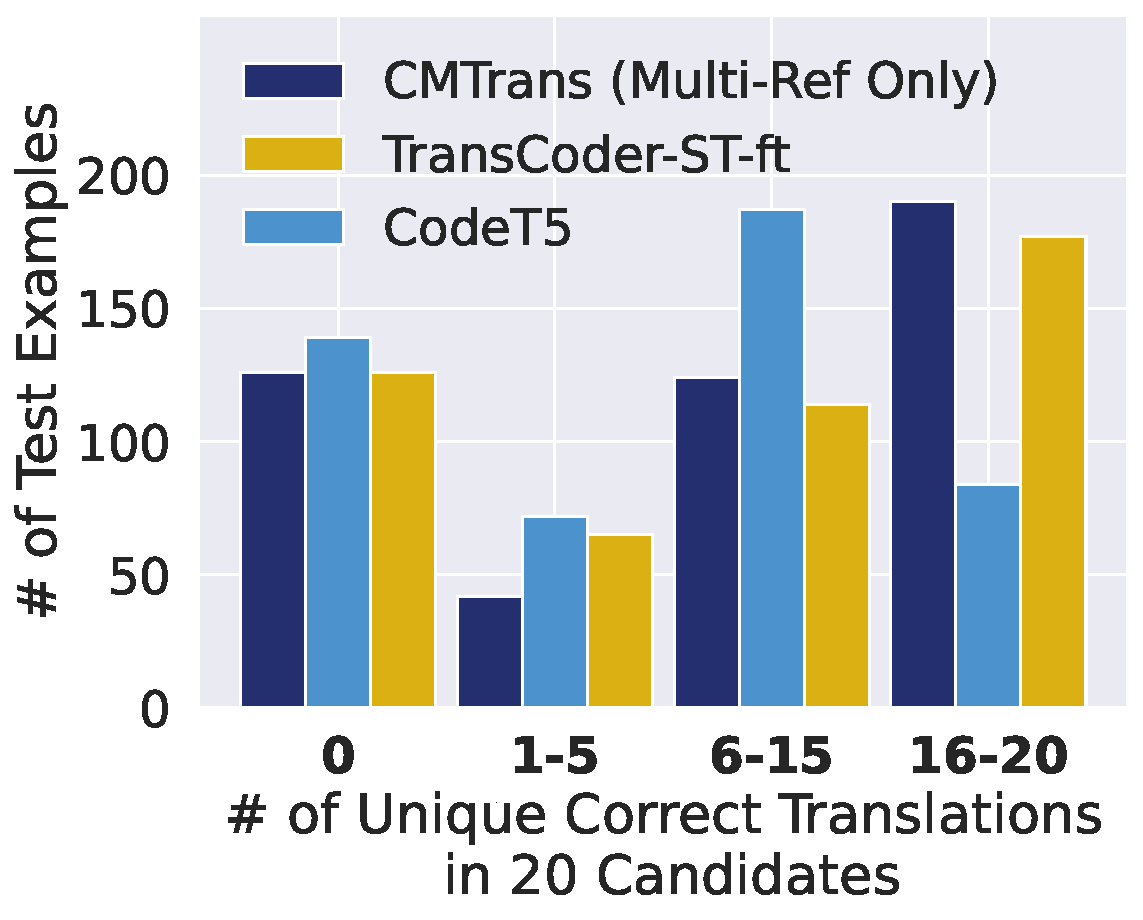
\includegraphics[width=\linewidth]{CMTrans_figs/unique_python2java.pdf}
  \caption{Python-to-Java}
  \label{fig:cmtrans_uni2}
\end{subfigure}
\caption{Number of unique correct translations in 20 candidates for each test example. We use beam search for each method, so the generated candidates are guaranteed to be distinct.}
\label{fig:cmtrans_unique}
\end{figure}




\begin{figure}
  \centering
  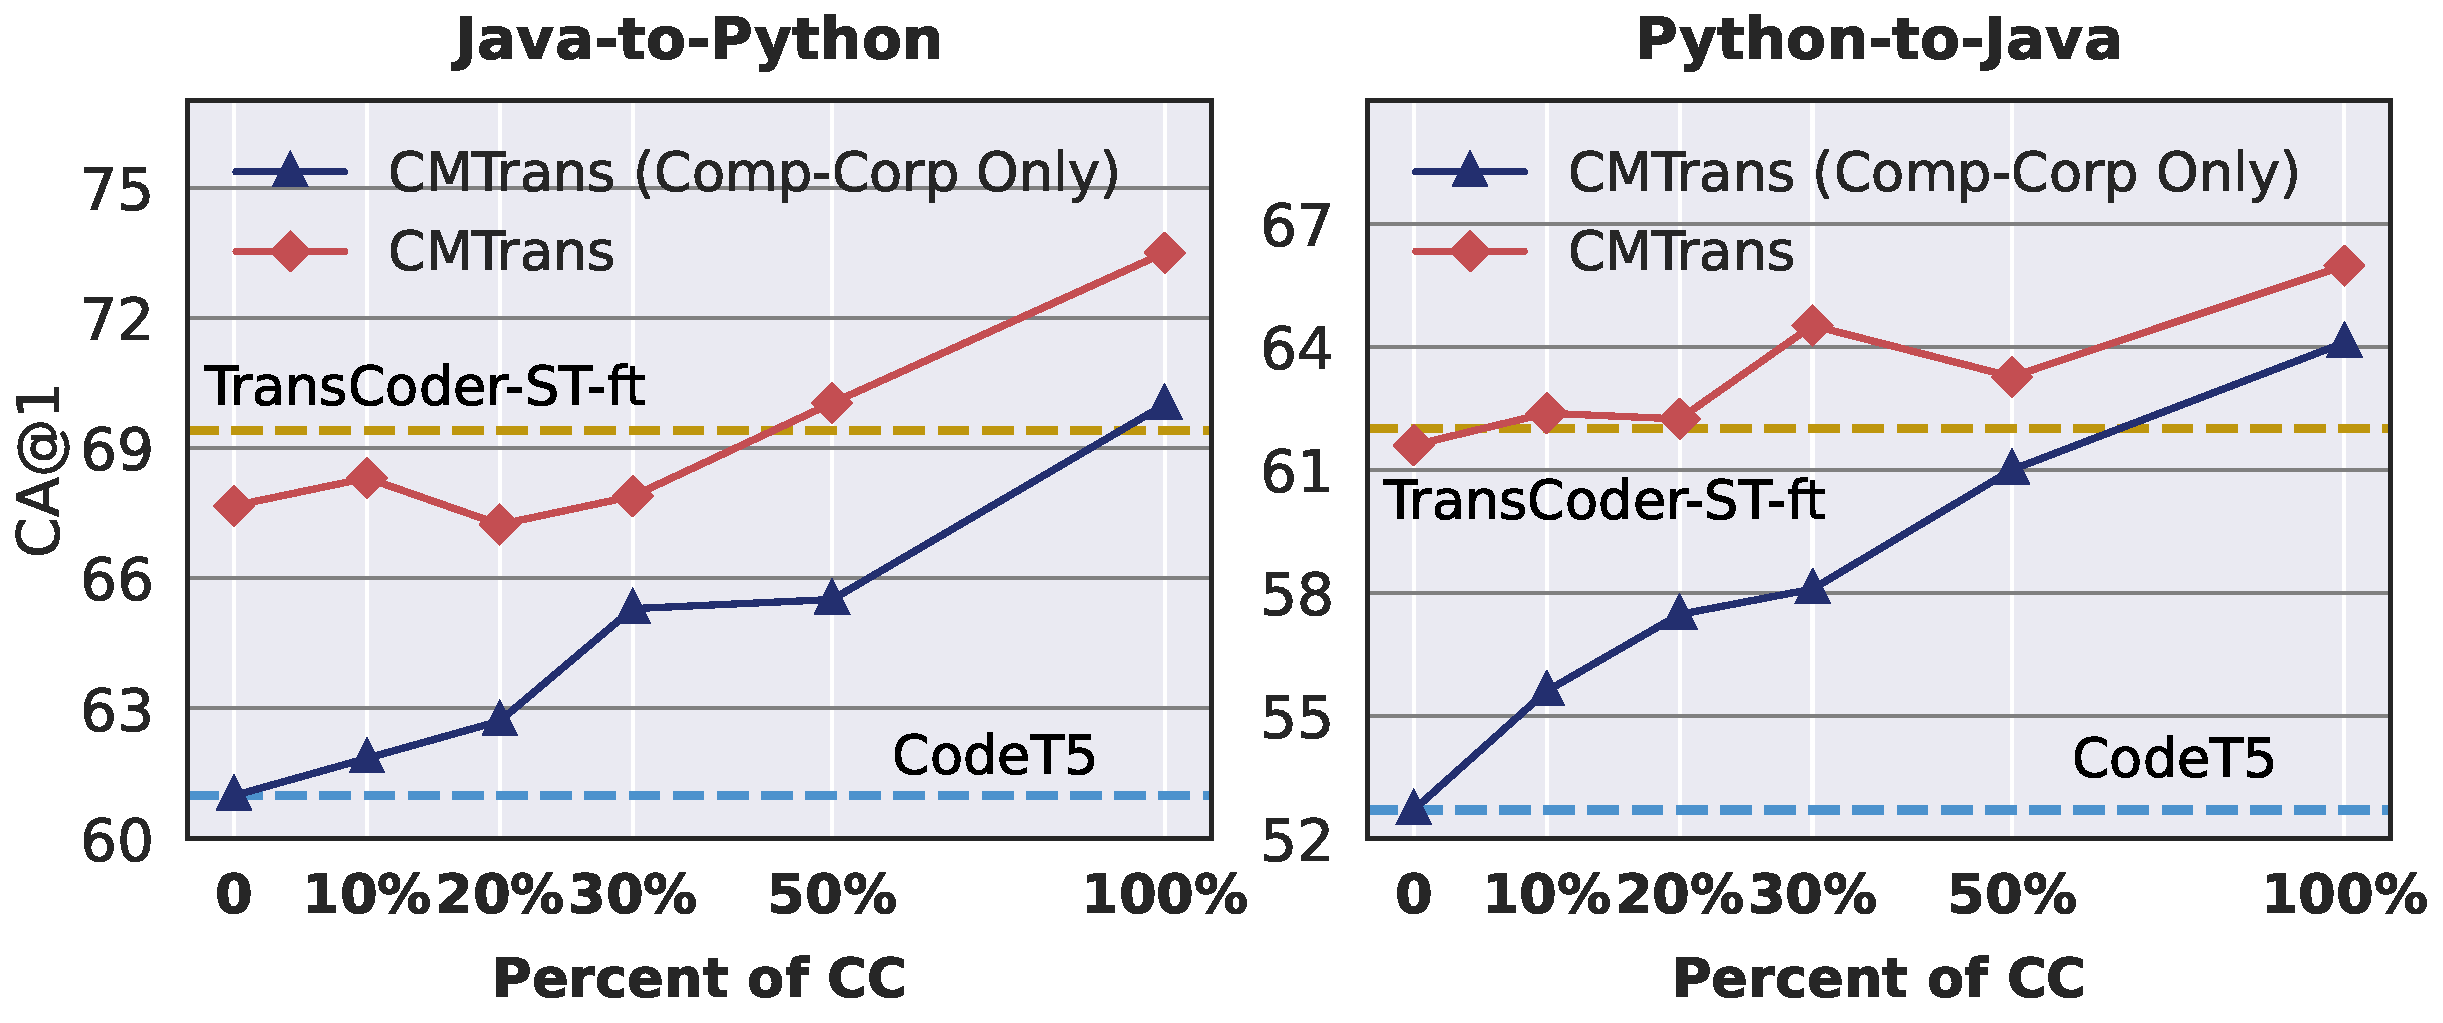
\includegraphics[width=0.7\linewidth]{CMTrans_figs/hyper_CC_analysis.pdf}
  \caption{Effect of the size of comparable corpora.}
  \label{fig:cmtrans_hyper_cc}
\end{figure}

\begin{figure}
  \centering
  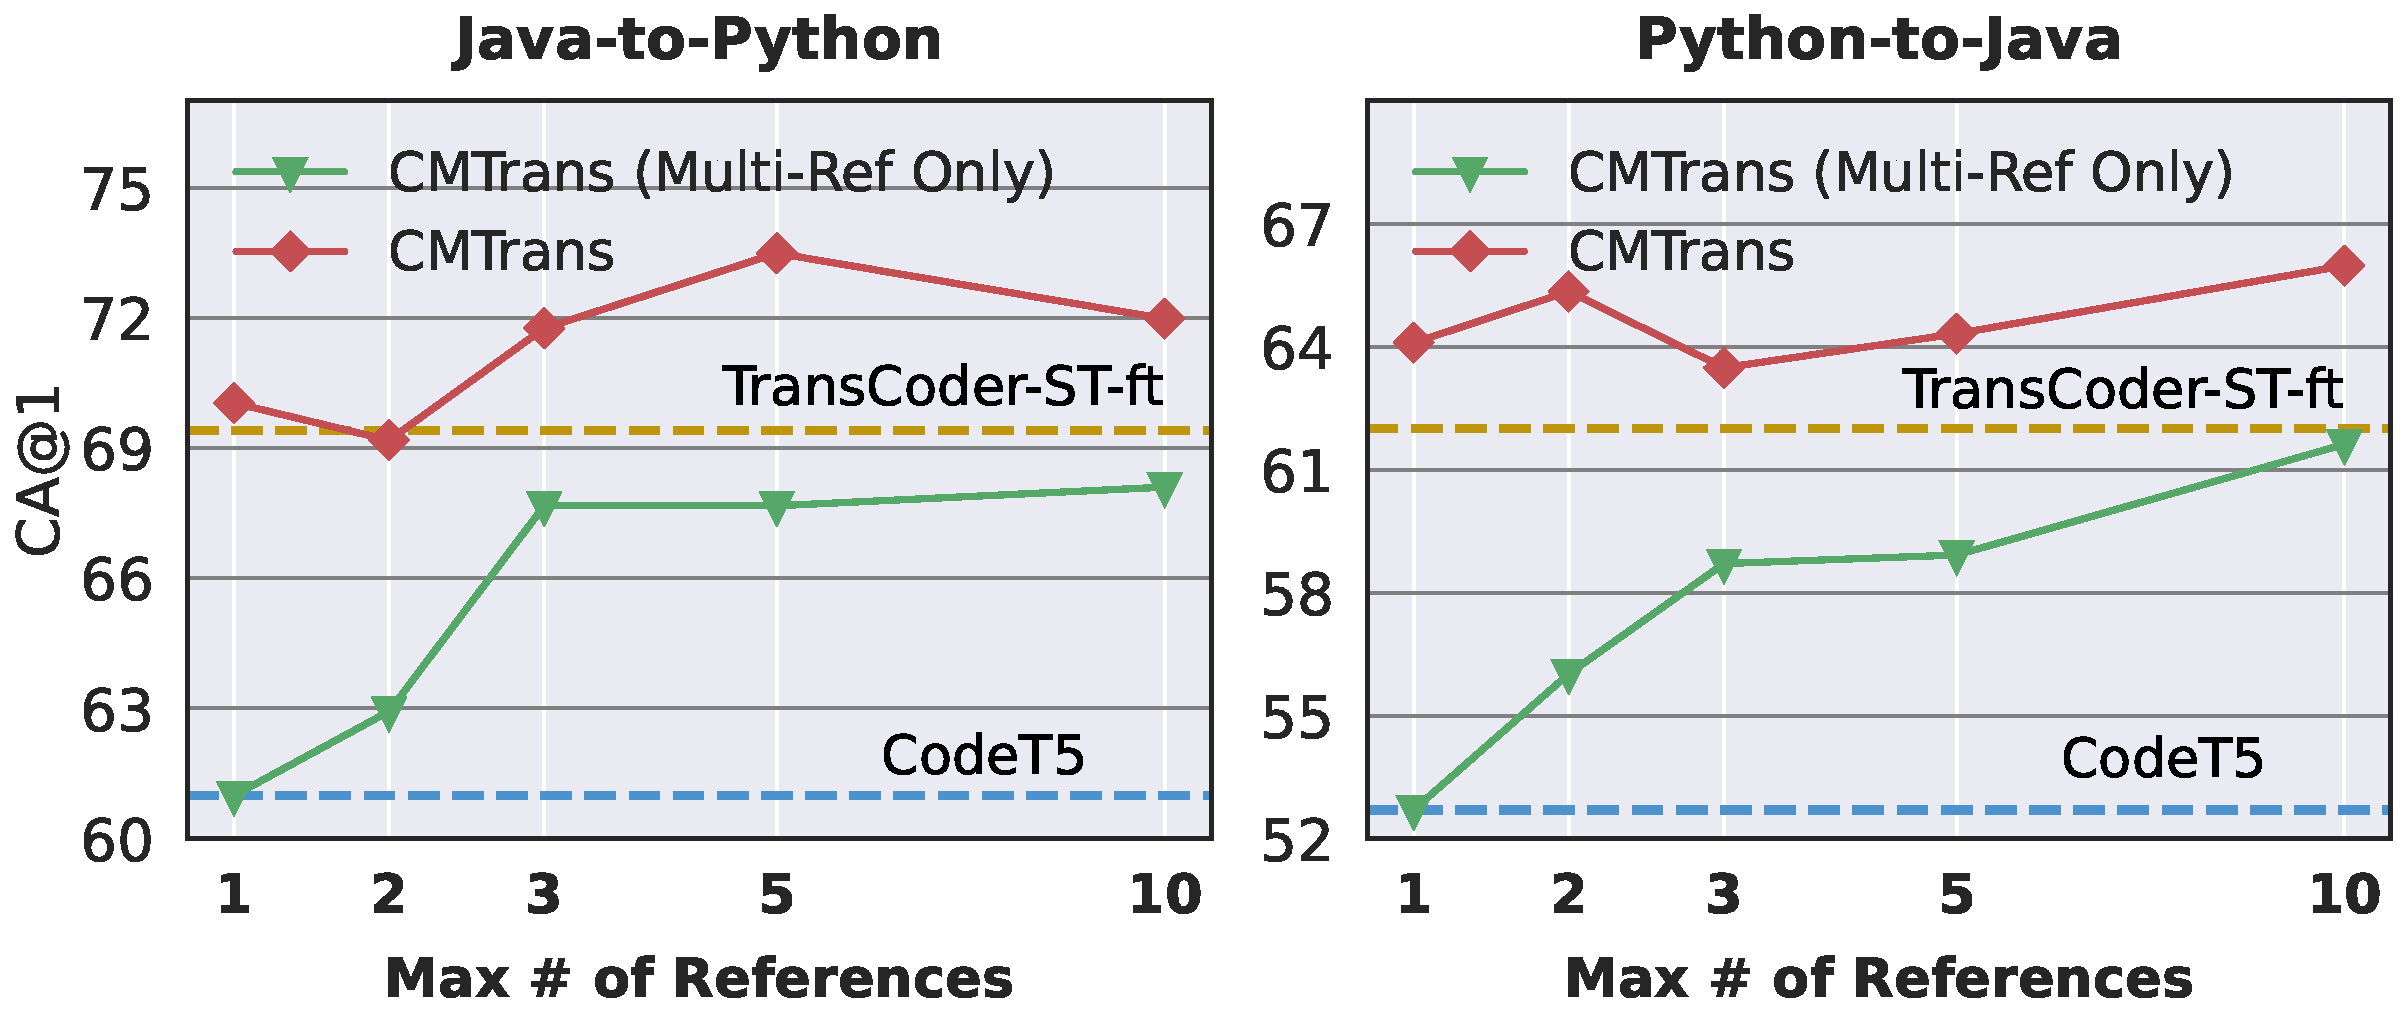
\includegraphics[width=0.7\linewidth]{CMTrans_figs/hyper_multi_analysis.pdf}
  \caption{Effect of the max number of references for each example.}
  \label{fig:cmtrans_hyper_multi}
\end{figure}

\subsection{Influence of Multiple References}
As for \textbf{RQ3}, we hypothesize that training on additional references can reduce overfitting to a single translation. 
To validate this hypothesis, we show in \autoref{fig:cmtrans_unique} that when trained with multiple references, \cmtransours can generate more unique correct translations using beam search within the same number of candidate outputs.
For instance, in Java-to-Python translation, there are 214 test examples where \cmtransours generates $\geq$ 16 unique translations, while there are only 145 and 146 examples for CodeT5 and TransCoder-ST-ft, respectively.
Furthermore, the scores under the ``0'' group indicate that after training with multiple references, the model generates at least one correct translation for more test examples.
In other words, in addition to CA@1, training CodeT5 on multiple references also improves on CA@20.

\subsection{Hyper-parameter analysis}
To answer \textbf{RQ4}, we analyze two hyper-parameters: 

\start{Size of comparable corpora}
We sample the same percentage of comparable examples from AVATAR-comp and Gen-comp and combine the sampled data.
\cmtransours is finetuned with at most 5 references in all trials.
As shown in \autoref{fig:cmtrans_hyper_cc}, as we increase the size of comparable corpora, \cmtransours (\CC Only) always has better performance.
While the trends are not monotonic for \cmtransours, it still obtains the best performance with full comparable corpora.

\start{Number of references}
We also examine the effect of the maximum number of references for each parallel example in finetuning.
We observe that the performance of \cmtransours does not always increase when finetuned with more references.
The reason might be that \cmtransours may generate more unique correct translations for some training examples than others.
As a result, the training signals the model received from different examples could be unbalanced, especially when the maximum number of references for each example is large.


\subsection{Case Studies}
We show a constructed comparable example in \autoref{fig:cmtrans_case}. 
% More case studies for comparable corpora and generated references can be found in Appendices~\ref{sec:app_case_cc} and \ref{sec:app_case_multi}.
As shown in \autoref{fig:cmtrans_case}, both the Java function extracted from GitHub and the generated Python function remove a config by name and return this config.
The only difference is the Java function obtains the name of each config by a helper function, while the generated Python function directly accesses the ``\texttt{name}'' attribute.
We also observe that this function is likely to belong to a large software project, which has a different nature from coding problems (e.g., the example in \autoref{fig:cmtrans_example_intro}).
As a result, combining collected and generated comparable examples provides diverse training signals to \cmtransours.

\begin{figure}[t]
    \centering
    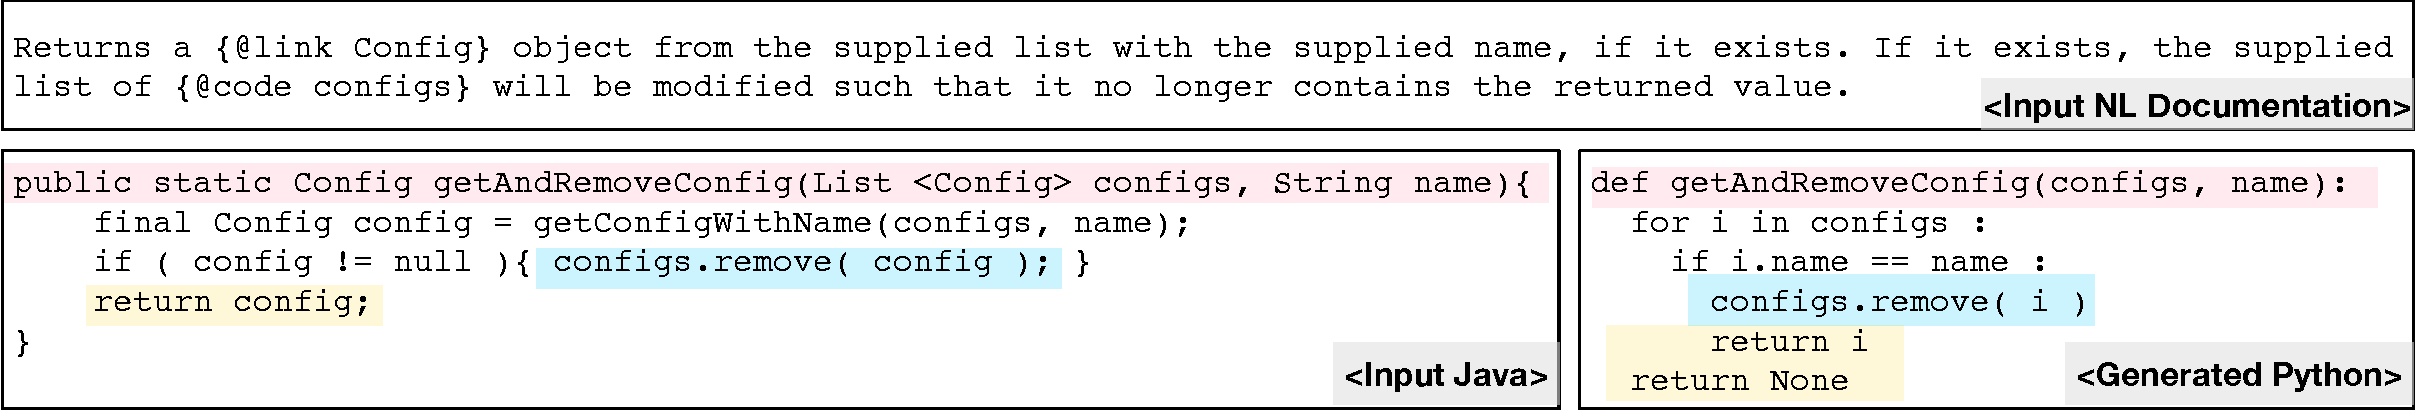
\includegraphics[width=\linewidth]{CMTrans_figs/case_short_fig_v2.pdf}
    \caption{Case study: a comparable example generated by our method with an NL-to-code generation model. We highlight the lines in the Java program and the generated Python program that can be matched.}
    \label{fig:cmtrans_case}
\end{figure}

\section{Chapter Summary}
In this chapter, we present two data augmentation techniques for code translation: comparable corpora and multiple references.
We study multiple ways of building comparable corpora, such as feeding natural language code documentation to code generation models.
Additionally, we generate multiple reference translations using \cmtransours and filter references using automatically generated unit tests.
Experiments on translation between 6 language pairs show that our two techniques improve CodeT5 substantially, by an average of 7.5\% CA@1.
The analyses further show that after training on comparable corpora, the model learns to generate more fluent code with the same types of constructs. With multiple references, the model learns to generate a larger number of unique correct translations.

While this chapter constructs scalable and effective training data for code translation, it focuses on \textbf{script-level} and \textbf{static} generation. Namely, the input and output are both code scripts, and the model generates code using one pass, without interacting with the environment.
The next chapter introduces the construction of scalable and effective training data for \textbf{repo-level} coding problems under the \textbf{coding agent} setting, which aims to generate code with real-world repositories as context. During inference, the model can interact with the environment by viewing files, editing files, executing bash commands, etc.. 






























\chapter{Constructing Scalable Coding Agent Training Environments with Sandbox Testing \textcolor{aquablue}{(\textit{completed})}}
\label{chap:repost}

\section{Introduction}
The previous chapter improves the scalability of script-level code translation data while remaining effective.
In this chapter, we construct scalable and effective repository-level (repo-level) coding agent training data by reducing the complexity of training environment construction.

% [motivate repo-level coding agent training]
Repo-level code generation aims to generate code with real-world, naturally occurring repositories as context, which aligns well with real-world software development.
However, most existing repo-level training datasets still treat code generation as a traditional sequence prediction task~\cite{codesearchnet,swebench}, neglecting the executable nature of code generation: the feedback can be obtained from execution.
In comparison, existing script-level code generation methods leverage execution feedback to improve model training~\cite{NEXT,plum,RLTF}.
They leverage online coding platforms as a natural resource to build large-scale algorithm problem datasets with test cases.
Such execution feedback is useful in constructing training targets~\citep{NEXT,plum} or reward signals~\citep{RLTF,exp_refine}.


While online coding platforms serve as a natural resource for large-scale algorithm problem datasets with test cases, it is non-trivial to build \textbf{execution-based} datasets for \textbf{repo-level} code generation at a \textbf{large scale}.
One major challenge is to set up executable environments.
Existing repo-level datasets typically conduct \textit{integration testing} that executes test files inside the repositories, which requires building the entire repository~\citep{swebench,R2E}.
As shown in prior research, this setup process is extremely challenging~\citep{super}, which may include installing external packages, determining execution context (e.g., relative import), debugging installation errors or runtime errors, etc.
Hence, existing methods for coding environment construction either require huge manual effort \citep{repocoder,swebench,swegym} or, when automated, suffer from low success rate~\citep{R2E}, limiting the scale of resulting datasets.

\begin{figure}
  \centering
  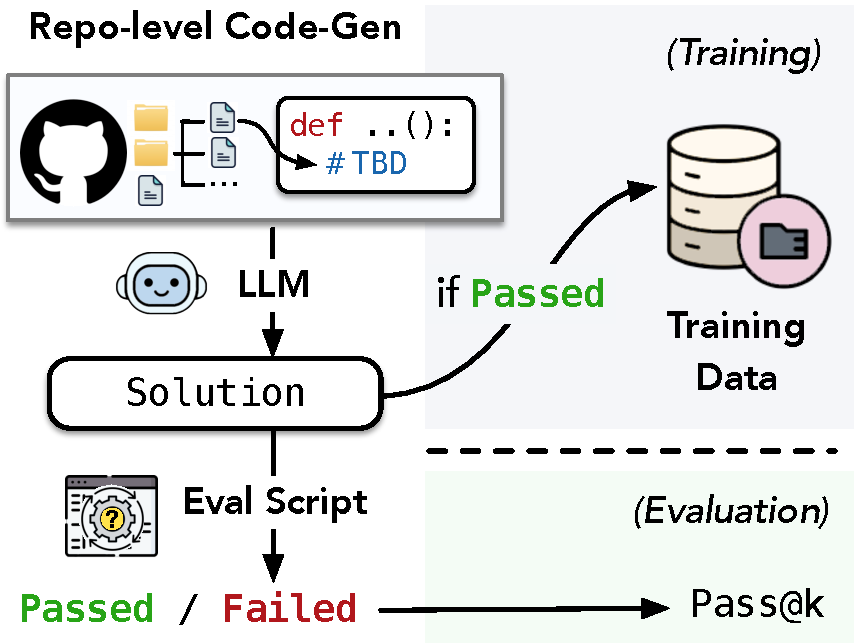
\includegraphics[width=0.6\textwidth]{RepoST_figs/intro.pdf}
  \caption{
    We can use the coding environments built by \repostmethodName for training and evaluation.
    We first apply the code generation model to generate candidate solutions with the original repository as context.
    Then we evaluate the solutions by executing the evaluation script built by \repostmethodName.
    For evaluation, we directly compute Pass@$k$ scores.
    For training, we add all successful solutions to the train set and further finetune the model.
  }
\label{fig:repost_intro}
\end{figure}

In this work, instead of integration testing, we present \repostmethodName, an \textbf{automated} framework to construct \textbf{Repo}-level coding environments with \textbf{S}andbox \textbf{T}esting.
Specifically, given a function in a GitHub repository, we sandbox the function and its local dependencies to a separate script and generate tests with an LLM.
To control the quality of the evaluation script, we iteratively resolve environment or runtime errors and improve test coverage.
We also conduct execution-based, AST-based, and LLM-based quality checks and only keep examples where the functionality of the sandboxed function does not alter and the tests are valid, reasonable, and have high coverage.
The resulting dataset allows us to obtain execution feedback in training and evaluation. 
As shown in \autoref{fig:repost_intro}, the models generate the target function with the entire GitHub repository as context. We then use the evaluation script to obtain execution feedback.

% [The method: RepoST]
Compared to integration testing used by previous datasets, we would like to highlight the benefits of sandbox testing in constructing \textbf{scalable} coding environments:
(1) In general, the external dependencies of a function are typically much simpler than those of a repository.
By isolating the function and its local dependencies, we can execute the function by \textit{only installing the necessary packages}.
(2) If any execution error occurs, we can debug the separate scripts \textit{without modifying the original repository}. This ensures that the datasets remain naturalistic: 
code generation models can still access the original, real-world repository.

% [Details of RepoST]
With the high scalability of our framework, we construct coding environment datasets for both training and evaluation: \reposttrainsetName and \repostevalsetName.
By the time the paper was published, \reposttrainsetName was the largest repo-level code generation dataset with execution support, with 7,415 functions sampled from 824 repositories.
The large scale enables training on \reposttrainsetName and evaluating on other benchmarks such as RepoEval~\citep{repocoder} or HumanEval~\citep{codex}.

% [Results on script-level code-gen]
Experiments show that by training on \reposttrainsetName, the method achieves performance gain on both algorithm problems in HumanEval~\citep{codex} and repo-level tasks in RepoEval~\citep{repocoder}.
For instance, we improve Qwen2.5-Coder by 5.5\% Pass@1 on HumanEval and 3.5\% Pass@1 on RepoEval and \repostevalsetName.

% [Results on SWE-Bench, SWT-Bench, and Commit-0, compared to the base model]
Note that \reposttrainsetName provides coding tasks based on real-world repositories that have execution feedback, it can also be applied to coding agent training~\citep{sweagent,openhands}.
For instance, after training on only 500 successful function generation trajectories sampled from \reposttrainsetName, we improve the resolved rates of Qwen2.5Coder-7B~\cite{qwen25coder} from 1.8\% to 7.8\% on the SWE-Bench issue-solving dataset~\cite{swebench}, from 0.23\% to 2.54\% on the SWT-Bench test generation dataset~\cite{swt-bench}, and from 4.80\% to 9.25\% on the Commit-0 library generation dataset~\cite{commit0}.


\section{Methodology}
The framework of \repostmethodName is illustrated in \autoref{fig:repost_framework}. 
After sampling GitHub repositories and extracting functions (\S\ref{sec:pre_curation}),
We sandbox each function and its local dependencies to a separate script (\S\ref{sec:sandboxing}), generate tests (\S\ref{sec:test_generation}), and conduct quality control on the executability of the scripts, the functionality of the sandboxed function, and the test quality (\S\ref{sec:quality_control}).
% We provide all the prompts in \S\ref{app:data-construction}.
When we use our environments to train (\S\ref{sec:code_gen_exps}) 
% and evaluate (\S\ref{sec:benchmarking_exps}) 
code generation models, the models can still access the original GitHub repository, and we provide execution feedback by executing the evaluation scripts.
To create user-friendly datasets, \textbf{we keep a shared Docker environment for all the evaluation scripts}.


\begin{figure}[t]
    \centering
    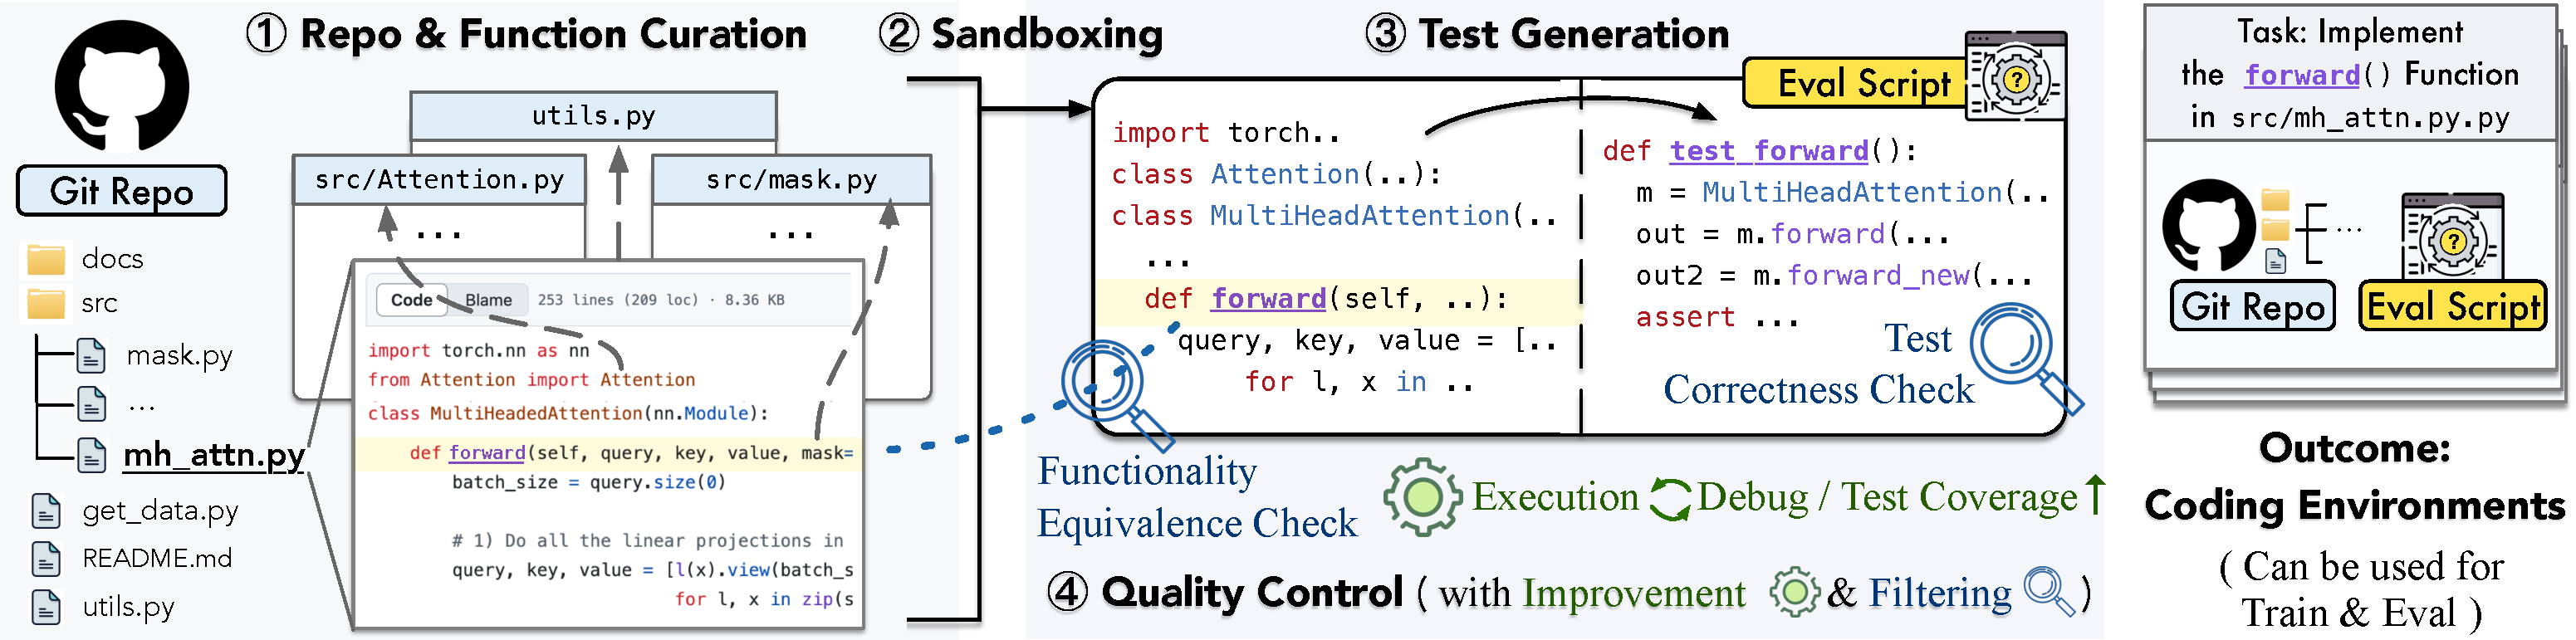
\includegraphics[width=\textwidth]{RepoST_figs/framework.pdf}
    \upv
    \caption{The \repostmethodName coding environment construction framework. We sandbox the target function and its dependencies to a separate evaluation script for execution, which avoids building the entire repository. We design careful quality control strategies with iterative quality improvement and post-filtering. The outcome of \repostmethodName is a set of executable repo-level coding environments, which can be used for training and evaluation.}
    \label{fig:repost_framework}
    \downv
\end{figure}


\subsection{Repository and Function Curation}
\label{sec:pre_curation}
We first randomly sample non-forked, MIT-licensed, Python GitHub Repositories with file sizes smaller than \texttt{10M}.
With the sandbox testing method, we are able to set up environments for individual functions and do not need to build the entire repository.
Hence, unlike previous works~\citep{R2E}, our method does not need to filter out repositories without setup files (e.g., \texttt{setup.py}).
The detailed repository statistics are provided in \S\ref{sec:dataset_stats}.


Then we extract functions from the repositories. 
To build the datasets in a docker with no access to GPUs or external services, we follow R2E~\citep{R2E} and filter out functions associated with GPUs, cloud tasks, etc. by keywords.
To balance the distribution of examples, we keep at most 30 functions for each repository.
After this step, for the train set, we started from 1,000 repositories and obtained 17,448 functions from 851 repositories.
For the evaluation set, we started from 200 repositories and obtained 1,043 functions from 139 repositories.
In theory, one can further scale up the dataset with more starting repositories.

\subsection{Sandboxing: Key to Environment Setup}
\label{sec:sandboxing}

\begin{figure}
  \centering
  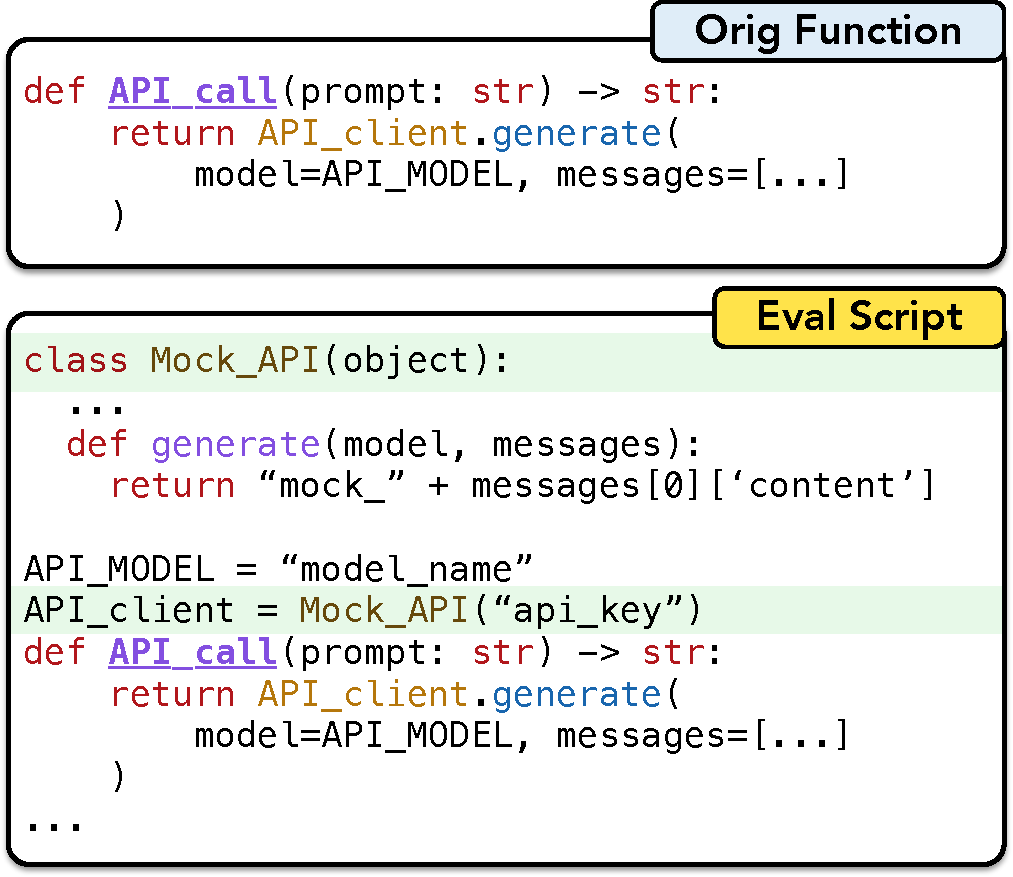
\includegraphics[width=0.6\linewidth]{RepoST_figs/sandboxing.pdf}
    \upv
  \caption{
    An example where the LLM successfully creates a mock class, \texttt{Mock\_API}, to replace real external API calls.
    In this way, while the function body of the target function \texttt{API\_call} remains exactly the same as in the original codebase,
    it can be executed without making real API calls.
  }
    \label{fig:repost_sandboxing}
    \downv
\end{figure}

It is non-trivial to create coding environments that provide correct execution feedback for the implementation of GitHub functions.
Existing methods typically provide execution feedback with integration testing, which creates test files that import the target function from the codebase. Executing such tests requires building the entire repository, which generally requires a complicated environment and is challenging for both human and LLMs.




With the observation that the external dependencies of a function are typically much simpler than a repository,
We tackle this challenge with \textbf{sandbox testing}, where we create a separate script containing the target function with the \textbf{exact same functionality} as the original one and the context that supports its executability.
By isolating the function and its local dependencies, we can execute the function by only installing the necessary packages.


\start{Sandboxing based on Local Dependencies}
The major challenge of sandboxing is to ensure the executability of the function.
While a standalone function can be directly copied to a separate script and executed, a typical GitHub function may depend on other modules, classes, or global variables in the same repository.
Thus, we leverage the call graph to extract such local dependencies that the target function directly or indirectly calls.
Then we combine all the code fragments into the context and prompt an LLM (e.g., GPT-4o) to aggregate all the code fragments into a single script, with as little editing as possible.


\start{Sandboxing External APIs and Files}
Even if all the dependencies are presented, it is still nontrivial to execute the sandboxed script if it requires external API, databases, files, etc. 
We explicitly prompt the LLM to create mock connections for any external API and create strings or write example files to a specific directory for file reading.
\autoref{fig:repost_sandboxing} presents a successful case of sandboxing with mock APIs.
% We provide examples of the generated sandboxed scripts in \Cref{fig:repost_case1-input,fig:repost_case1-sandbox,fig:repost_case1-tests,fig:repost_case2-input,fig:repost_case2-sandbox,fig:repost_case2-tests}.
% % \S\ref{app:case-studies}.


\start{Functionality Equivalence Control}
In addition to executability, another challenge of sandboxing is to ensure that the target function's functionality does not alter.
We first conduct a list of sanity checks on the function name, length of scripts, etc., and re-generate examples that do not satisfy the requirements.
We also have a final quality control step (in \S\ref{sec:quality_control}) that compares the functionality of the sandboxed and original functions.
The precision of quality control is further verified in the human study in \S\ref{sec:human_study}.


\subsection{Test Generation}
\label{sec:test_generation}

\start{Equivalence Testing}
We generate synthetic tests in the sandboxed script to evaluate the correctness of the generated code.
Specifically, we prompt the LLM to (1) generate a set of test inputs to the target function and (2) conduct equivalence testing that checks whether the function generated in evaluation has the same behavior as the sandboxed function (i.e., the ``ground-truth'' implementation).
Compared to traditional methods that specify the I/O examples in the test cases~\citep{codex}, equivalence testing does not need to predict the expected outputs and is more feasible for LLMs~\citep{R2E}.


\start{Test Generation with Mock APIs and Files}
We observe that the LLM is able to generate tests with the mock classes created in the sandboxing step as context. 
% As shown in \Cref{fig:repost_case2-input,fig:repost_case2-sandbox,fig:repost_case2-tests}, 
As shown in \autoref{fig:repost_sandboxing}, we create mock class instances as the test inputs and still ensure that the function body of the sandboxed function remains the same as the original function.

\start{Test Quality Control}
Similarly to the sandboxing step, for quality control purposes, we conduct a series of sanity checks, such as requiring the test function to call the target function and have at least 3 assertions.
% (see \autoref{tab:sanity_check_test_gen} for the full list). 
We further check the coverage and correctness of the tests in the final quality control step (\S\ref{sec:quality_control}), 


\subsection{Quality Control and Filtering}
\label{sec:quality_control}

We conduct quality control for the executability of the evaluation script, the functionality of the sandboxed function, and the test quality.

\start{Iterative Execution and Debugging}
In principle, if the model-generated function is exactly the same as the ground truth, the evaluation scripts should be successfully executed, with all the tests passed.
Hence, we execute the examples sequentially in a docker. If there are any execution errors or if the ground truth implementation cannot pass any test cases, we provide the error message as the context and prompt an LLM to debug the evaluation script. Examples that still have errors after $k$ execution-debugging iterations are filtered out.

We also dynamically install external packages during execution.
During execution, if there are any \texttt{ModuleNotFound} errors, we extract the package names from the error message, run a \texttt{pip install} command, and execute the script again.
In case the package name differs from the import name or the code requires a specific version of packages, we also allow the LLM to output package installation commands during debugging.
In this way, we are able to install external packages for functions extracted from repositories without setup files.


\start{Iterative Test Coverage Improvement}
To ensure that the test functions cover the major functionality of the target functions, we further compute the branch coverage rate of all the evaluation scripts.
If the branch coverage rate is lower than some threshold (we set $80\%$ for the train set and $100\%$ for the evaluation set),
We provide the LLM with the missing lines and prompt it to improve the test function by incorporating more tests.


\start{Final-Step Quality Check \& Filtering}
As a final step, we conduct two quality checks: functionality equivalence check and test correctness check, and filter out unqualified examples. 


To ensure the validity of sandbox testing, we examine the \textbf{functionality equivalence} between the sandboxed and original function.
We first compare the AST of the function bodies, which is a sufficient condition of functionality equivalence. 
In our resulting dataset, 81.7\% of the examples have the same AST. The remaining ones are filtered out from the evaluation set. 
To include more examples in the train set, 
since it is also possible that code with the same functionality has different ASTs (e.g., HTML tags can be parsed with \texttt{LexborHTMLParser} and \texttt{BeautifulSoup}),
We prompt an LLM~\footnote{The original code could be inexecutable due to package installation errors (e.g., \texttt{BeautifulSoup} in this case), so we do not execute the original code.} to compare the functionality equivalence, which is shown to have high agreement with human (see our human study in \S\ref{sec:human_study} for details).
We also include the examples that pass the LLM check for the train set.


In principle, a test that calls the target function without any assertion checks still has a 100\% coverage rate.
We hence conduct \textbf{test correctness} check and apply an LLM to check whether the tests are correct, reasonable, and complete the verification of the functionality. Human study in \S\ref{sec:human_study} demonstrates the high precision of the LLM test correctness checker.


\begin{table}[t]
\centering
\resizebox{0.7\linewidth}{!}{
\begin{tabular}{lrrcc}
\toprule
\textbf{Dataset} & \textbf{\#Ex} & \textbf{\#Repo} & \textbf{Repo?} & \textbf{AutoTest?} \\
\midrule
HumanEval & 164 & -- & \xmark & \xmark \\
DS1000 & 1,000 & -- & \xmark & \xmark \\
ClassEval & 100 & -- & \xmark & \xmark \\
RepoEval-Func & 455 & 6 & \cmark & \xmark \\
SWE-Bench & 2,294 & 12 & \cmark & \xmark \\
CoderEval & 230 & 43 & \cmark & \xmark \\
DevEval & 1,874 & 117 & \cmark & \xmark \\
EvoCodeBench & 275 & 25 & \cmark & \xmark \\
SWE-Gym & 2,438 & 11 & \cmark & \xmark \\
R2E-Eval1 & 246 & 137 & \cmark & \cmark \\
R2E (Reproduced) & 744 & 123 & \cmark & \cmark \\
\midrule
\textbf{\reposttrainsetName} & \textbf{7,415} & \textbf{824} & \cmark & \cmark \\
\textbf{\repostevalsetName} & 296 & 99 & \cmark & \cmark \\
\bottomrule
\end{tabular}
}
\caption{Statistics of \reposttrainsetName and \repostevalsetName compared to existing \textbf{execution-based} code generation datasets. 
R2E (Reproduced) applies the R2E method to the same set of input repositories as \reposttrainsetName, but results in a smaller number of repositories and examples.
``Repo?'' and ``Auto Test?'' refer to the repo-level setting and automatically generated tests.}
\label{tab:repost_stats}
\end{table}

\begin{table}[t]
\centering
\resizebox{0.7\textwidth}{!}{
\begin{tabular}{lcc}
\toprule
\bf Avg Stats.
& \textbf{\textsc{Train}} 
& \textbf{\textsc{Eval}} \\
\midrule
Target \# Tokens (Lines) & 112.4 (12.8) & 102.7 (9.9) \\
Eval Script \# Tokens (Lines) & 842.5 (75.7) & 1217.5 (122.3) \\
\# Test Cases & 5.7 & 8.2 \\
Test Branch Coverage & 97.8\% & 100\% \\
\% Standalone Functions & 28.1\% & 26.4\% \\
\# External Libraries & 894 & 106 \\
\bottomrule
\end{tabular}
}
\caption{Detailed statistics of our datasets.}
\label{tab:repost_detailed_stats}
\end{table} 


\begin{table}[t]
\centering
\resizebox{0.4\linewidth}{!}{
\begin{tabular}{l|cc|cc}
\toprule
\textbf{Check} & \multicolumn{2}{c|}{\textbf{Func}} & \multicolumn{2}{c}{\textbf{Test}} \\
\cmidrule(lr){2-3} \cmidrule(lr){4-5}
Human $\rightarrow$ & Yes & No & Yes & No \\
\midrule
GPT-4o: Yes & 13 & 0 & 9 & 1 \\
GPT-4o: No & 1 & 6 & 4 & 6 \\
\bottomrule
\end{tabular}
}
\caption{Agreement between human and GPT-4o on checking (1) the functionality equivalence between the sandboxed and original function, and (2) the test correctness.
When GPT-4o predicts ``Yes'' for both quality checks, it has a high agreement with human.}
\label{tab:repost_agreement}

\end{table}

\begin{table}[t]
\centering
\resizebox{0.5\linewidth}{!}{
\begin{tabular}{ccc}
\toprule
\textbf{\% Solved} & \textbf{\% Use-Tool} & \textbf{Easy / Med / Hard} \\
\midrule
81.5\% & 59.3\% & 29.6 / 51.9 / 18.5 \\
\bottomrule
\end{tabular}
}
\caption{Human study results. We ask the participants to complete the function with the same context we use to evaluate code generation models in \S\ref{sec:code_gen_exps}.}
\label{tab:repost_human_study_1}
\end{table}




\section{Resulting Datasets: \reposttrainsetName and \repostevalsetName}
\label{sec:dataset_stats}

\start{Statistics}
We build a train set, \reposttrainsetName, and an evaluation set, \repostevalsetName.
To reduce contamination, we build \reposttrainsetName from repositories created between \texttt{2023-01-31} and \texttt{2024-08-31},
and build \repostevalsetName from repositories created after \texttt{2024-09-01}.


We compare the statistics of the datasets and existing \textit{execution-based} datasets in \autoref{tab:repost_stats}.
By the time the paper was published, \reposttrainsetName was the largest repo-level dataset with execution feedback.
Prior works such as RepoEval~\citep{repocoder} or SWE-Gym~\citep{swegym} require huge human effort to set up the environments.
Automated frameworks such as R2E~\citep{R2E} apply LLMs to the complicated task of building the entire repositories and suffer from low success rates.
In comparison, \repostmethodName only requires necessary dependencies for each function, which is more feasible for LLMs and benefits scalability.




\autoref{tab:repost_detailed_stats} shows detailed statistics of our datasets.
Our datasets achieve high test numbers and branch coverage rates with iterative test coverage improvement and quality filtering.
Results also show that \repostmethodName can create relatively complex examples in terms of length and local and external dependencies.
The percentage of standalone functions (i.e., functions without local dependencies) are 28.1\% and 26.4\% in our datasets. Both are very close to 27\%, the percentage of standalone functions among all GitHub code estimated by \citet{deveval}.





\subsection{Quality Verification with Human Study}
\label{sec:human_study}

\start{Agreement between LLM Checker and Human}
We conduct a human study to verify the precision of our LLM-based quality check strategies introduced in \S\ref{sec:quality_control}.
We ask 3 computer science graduate students to conduct functionality equivalence and test correctness checks for
20 examples sampled from \repostevalsetName (before the final filtering), with the same instruction we use to prompt the LLM checkers.
The Kappa agreement scores among human annotators are 0.9179 for the functionality check and 0.7750 for the test check.

Results in \autoref{tab:repost_human_study_1} show that all 13/20 examples that pass GPT-4o's functionality check are also predicted as ``same functionality'' by human.
Among 10 examples that pass GPT-4o's test quality check, 9 of them are predicted as ``high-quality tests'' by human.
It demonstrates that after applying our filtering strategies for quality control, the remaining examples have high quality.
In principle, one can further enhance dataset quality by manually inspecting and selecting the examples.
% We provide more details about the experiments in \S\ref{app:human-study-details}.





\start{Solvability Check}
We conduct another human study to check whether the examples are reasonable and can be solved by human.
We assigned 27 examples constructed by \repostmethodName to 9 computer science students, with no overlaps, and asked them to complete the function and answer questions about the difficulties of the examples.
% (see \S\ref{app:human-study-details} for details).

Results show that 81.5\% of the examples were solved by human, indicating that most examples are reasonable and not too complicated.
The remaining examples were not solved for various reasons, such as the participant is not familiar with the task (e.g., reading html data) or related libraries (e.g., \texttt{BeautifulSoup4}), the intent of the function cannot be fully entailed from the context, etc.
% Towards the unclear intent issue, we designed an experiment in \S\ref{sec:benchmarking_exps}, where we generated additional instructions to improve the clarity.
We also observe that the generated examples have varying complexity levels based on the usage of external tools and the difficulty ratings.
Furthermore, 33.3\% of the examples
are solved in the first submission and 37.0\% require more than 5 submissions to solve. 




\section{Code Generation Training Experiments}
\label{sec:code_gen_exps}
\start{Training with \reposttrainsetName} 
In standard supervised fine-tuning (\textbf{SFT}), we can train the model with the code context $c$ as the input and the ground truth target function $f^*$ as the output.
The execution feedback provided by our \repostmethodName evaluation scripts further allows us to employ the \textbf{rejection sampling fine-tuning (RFT)} algorithm to generate additional valid training targets.
Specifically, we apply the model itself to our dataset, generating $n$ candidate solutions for each function based on its code context: $(c, f_1), \ldots (c, f_n)$. The method is denoted as \textbf{RFT (Self)}.
We can also apply other stronger models to generate candidates (denoted as \textbf{RFT (Distill)}). 
Only solutions that pass our test cases are retained.
We then finetune the model on the successful functions $(c, f_1'), \ldots (c, f_m')$ and the ground truth $(c, f^*)$ using the standard negative log-likelihood loss.

To obtain more training pairs for both the ``Self'' and ``Distill'' settings, we further prompt the model itself or a stronger model to debug the failed solutions, with the error message in the context.
We also train the model on successfully debugged solutions $(c, f_1''), \ldots (c, f_k'')$.





\begin{table}[t]
\centering
\resizebox{0.8\textwidth}{!}{
\begin{tabular}{lcccccc}
\toprule
\multirow{2}{*}{\textbf{Model}}  
& \multicolumn{2}{c}{\bf HumanEval} 
& \multicolumn{2}{c}{\textbf{RepoEval-Func}} 
& \multicolumn{2}{c}{\bf \repostevalsetName} \\
\cmidrule(lr){2-3}
\cmidrule(lr){4-5}
\cmidrule(lr){6-7}
& Pass@$1$ & $\Delta$ & Pass@$1$ & $\Delta$ & Pass@$1$ & $\Delta$ \\
\midrule
StarCoder2-7B~\citep{starcoder2} 
& 34.76 & -- & 32.98 & -- & 26.35 & -- \\
\quad + SFT 
& 37.20 & \small{\colordg{$\uparrow$2.44}} 
& 33.78 & \small{\colordg{$\uparrow$0.80}}
& 27.70 & \small{\colordg{$\uparrow$1.35}} \\
\quad + RFT (Self) 
& 39.63 & \small{\colordg{$\uparrow$4.87}}
& 34.58 & \small{\colordg{$\uparrow$1.61}}
& 28.38 & \small{\colordg{$\uparrow$2.03}} \\
\quad + RFT (Distill) 
& \textbf{40.24} & \bf \small{\colordg{$\uparrow$5.49}}
& \textbf{35.12} & \bf \small{\colordg{$\uparrow$2.14}}
& \textbf{29.05} & \bf \small{\colordg{$\uparrow$2.70}} \\
\midrule
Qwen2.5-Coder-7B~\citep{qwen25coder} 
& 79.27 & -- & 38.06 & -- & 29.39 & -- \\
\quad + SFT 
& 80.48 & \small{\colordg{$\uparrow$1.21}} 
& 39.94 & \small{\colordg{$\uparrow$1.88}} 
& 30.74 & \small{\colordg{$\uparrow$1.35}} \\
\quad + RFT (Self) 
& \bf 84.76 & \bf \small{\colordg{$\uparrow$5.49}} 
& 40.75 & \small{\colordg{$\uparrow$2.69}} 
& 31.76 & \small{\colordg{$\uparrow$2.36}} \\
\quad + RFT (Distill) 
& \bf 84.76 & \bf \small{\colordg{$\uparrow$5.49}} 
& \bf 41.55 & \bf \small{\colordg{$\uparrow$3.49}} 
& \bf 32.43 & \bf \small{\colordg{$\uparrow$3.04}} \\
\bottomrule
\end{tabular}
}
\caption{Code generation training results. We evaluate Pass@1 for all experiments. For RepoEval, we use the ``Oracle'' repo-level context as used in their original paper.
}
\label{tab:repost_main}
\end{table}


\subsection{Experimental Setup} 
\start{Datasets and Evaluation Metrics}
We train two models: StarCoder2-7B~\citep{starcoder2} and Qwen2.5-Coder-7B~\citep{qwen25coder} with \reposttrainsetName and evaluate on two public benchmarks: HumanEval~\citep{codex}, an algorithm problem dataset, and RepoEval~\citep{repocoder}, a repo-level code generation dataset. We also evaluate on \repostevalsetName.
For RepoEval, we only evaluate on the ``function'' split, which supports execution. We use the ``Oracle'' context to mitigate the bias of context retrieval methods.
We report the Pass@1 scores on all datasets.
% More evaluation details are provided in \S\ref{app:training-exp-details}.


\start{Training Details}
We compare three training methods: SFT, RFT (Self), and RFT (Distill).
For the ``Distill'' method, we apply GPT-4o and Claude-3.5-Sonnet to generate and debug candidate solutions, separately, and combine their successful candidates for training.
% We provide the number of examples where we obtained at least one successful solution in \autoref{tab:rej_sampling_stats}.
% Other details are shown in \autoref{app:training-exp-details}.


\subsection{Experimental Results}
\start{Main Results}
\autoref{tab:repost_main} demonstrates that models trained with \reposttrainsetName can generalize well to other public benchmarks.
Specifically, we improve Qwen2.5-Coder by 5.5\% Pass@1 on HumanEval, 3.5\% on RepoEval-Func, and 3.0\% on \repostevalsetName.
Furthermore, in all experiments, training with RFT, even with self-training only, achieves better performance than finetuning on the original GitHub function only.
For instance, RFT (Distill) outperforms SFT by 4.3\% Pass@1 on HumanEval.
This shows the benefit of training with environments that can provide execution feedback.
We can also observe that RFT with self-training in general has lower performance than distilling from stronger models. 
% As shown in \autoref{tab:rej_sampling_stats}, 
Particularly,
We can only obtain 1573 additional training targets with StarCoder2, but we obtained 3606 by combining GPT-4o and Claude-3.5.
We hypothesize that one can obtain more examples and hence achieve better performance by sampling with more candidate solutions, generating from different types of context, etc., and we leave that to future work.




\start{Scaling Law Analysis}
In \autoref{fig:repost_scaling_law}, we investigate how the scale of training data affects model performance. 
Specifically, we randomly sample different numbers of examples from \reposttrainsetName to train the model.
We can see that the performance of RFT (Distill) increases as we scale up the training data, which suggests the advantage of training data with high scalability.
Furthermore, with different scales of data, RFT consistently achieves better performance than SFT, which further demonstrates the effectiveness of training environments with execution feedback.



\begin{figure}
  \centering
  \begin{subfigure}[b]{0.4\textwidth}
    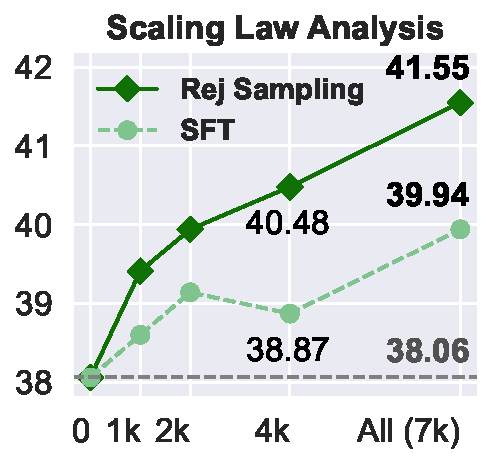
\includegraphics[width=\textwidth]{RepoST_figs/scaling_law.pdf}
    \caption{Scaling law analysis.}
    \label{fig:repost_scaling_law}
  \end{subfigure}
  \hspace{0.4cm}
  \begin{subfigure}[b]{0.32\textwidth}
    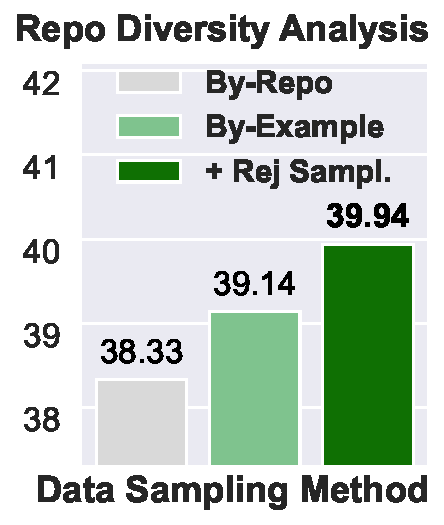
\includegraphics[width=\textwidth]{RepoST_figs/repo_diversity.pdf}
    \caption{Repo diversity.}
    \label{fig:repost_diversity_study}
  \end{subfigure}
  \caption{(a) Pass@1 scores on RepoEval with different numbers of training examples.
  (b) Pass@1 scores on RepoEval with different methods to sample 2,000 training examples. 
  Sample-by-Example has a broader repository coverage and achieves better Pass@1. The performance is further enhanced with RFT (Distill).
  }
  \label{fig:repost_analysis}
\end{figure}


\start{Repository Diversity Experiment}
\autoref{fig:repost_diversity_study} examines whether broader repository coverage leads to better performance, given a fixed budget of training examples.
We fix the number of examples to 2,000 and experiment with two example sampling methods: (1) Sample-by-Repo, where we keep sampling repositories and adding all the functions in the repository to the training set, until the data size reaches 2,000; (2) Sample-by-Example, which is the same setting as \autoref{fig:repost_scaling_law}, where we randomly sample functions from \reposttrainsetName.
We observe that Sample-by-Example, covering 678 repositories, outperforms Sample-by-Repo, which only covers 221. The performance is further improved by RFT.
Recall that our method only needs to set up individual functions, compared to existing methods, such as R2E, that need to build the entire repository, it is much easier to build datasets with broad repository coverage with our method, which benefits model training.




\section{Coding Agent Training Experiments}
In this section, we show that in addition to static code generation models, \reposttrainsetName can also be used to train coding agents.

\subsection{Experimental Setup}
\start{Training Coding Agents with \reposttrainsetName}
We formulate the training task as follows: given a GitHub repository and the path to a function in it, whose body has been masked out, the agent needs to implement this function based on a piece of textual description.

To set up the task, we run a Docker container for each \reposttrainsetName instance. We clone the GitHub repository and checkout to the specific commit. The target function would be masked properly before applying the agent to solve the task.
Then we apply the agent to complete the masked function.
After it finishes, we extract the function body it generates (if any), and run \repostmethodName's evaluation script to verify its correctness.

Finally, similar to \autoref{sec:code_gen_exps}, we train the agent model with rejection sampling finetuning: we apply the teacher model on a set of training instances, evaluate the results, and train the model on the collection of successful trajectories with supervised finetuning.

\start{Training Details}
In this experiment, we use Claude-3.7~\cite{claude37} as the teacher model and train Qwen2.5-Coder-7B as the student model. We use OpenHands~\cite{openhands} (v0.40.0) as the agent scaffold.
To limit the cost of generating training trajectories, we only generate 500 successful trajectories with Claude-3.7 for training.

\start{Evaluation Datasets and Metrics}
We report the resolved rates on three repo-level coding agent benchmarks: the SWE-Bench Verified issue-solving benchmark~\cite{swebench}, the SWT-Bench Verified test generation benchmark~\cite{swt-bench}, and the Commit-0 library construction benchmark~\cite{commit0}.
Note that none of the benchmarks specifically targets function generation. Namely, the experiment is under the zero-shot task generalization setting.

\subsection{Experimental Results}
\autoref{tab:repost-agent} presents the results of training the Qwen2.5-Coder-7B agent on 500 trajectories generated from \reposttrainsetName.
Results show that although \reposttrainsetName does not target issue-solving, test generation, or library construction, the finetuned agent significantly outperforms the base model in all three benchmarks.
Particularly, we improve the performance of Qwen2.5Coder-7B from 1.8\% to 7.8\% on SWE-Bench Verified, from 0.23\% to 2.54\% on SWT-Bench Verified, and from 4.80\% to 9.25\% on Commit-0 Lite.
This demonstrates that the \repostmethodName training environments are also effective in training coding agents.
Note that we only train the agent on 500 successful trajectories (generated from around 1200 \reposttrainsetName instances) due to computational budget.
It is possible to generate a larger training set based on the entire \reposttrainsetName dataset. We leave the exploration to future work.


\begin{table}[t]
\centering
\small
\resizebox{0.8\columnwidth}{!}{%
\begin{tabular}{l ccc}
\toprule
\bf Methods & \bf SWE-Bench & \bf SWT-Bench & \bf Commit-0 \\
 & Resolved \% & Resolved \% & Resolved \% \\
\midrule
Qwen2.5Coder-7B & 1.8 & 0.23 & 4.80 \\
+ \reposttrainsetName (500) RFT 
& \bf 7.8~{\textcolor{treegreen}{$\uparrow$6.0}} 
& \bf 2.54~{\textcolor{treegreen}{$\uparrow$2.31}} 
& \bf 9.25~{\textcolor{treegreen}{$\uparrow$4.45}} \\
\bottomrule
\end{tabular}%
}
\caption{Performance of the Qwen2.5Coder-7B agent on SWE-Bench Verified, SWT-Bench Verified, and Commit-0 Lite before and after training. 
}
\label{tab:repost-agent}
\end{table}








% \section{Related Work}

% \start{Code Generation Training}
% Existing works have shown the effectiveness of pretraining~\citep{codellama,starcoder2,deepseekcoder} or instruction tuning~\citep{wei2023magicoder,wizardcoder,dsR1} on real-world code.
% To further finetune models for code generation, existing works have built large-scale training datasets with test cases by leveraging large-scale online algorithm problems.
% The execution feedback from test cases is used in constructing training targets~\citep{NEXT,plum} or reward signals~\citep{RLTF,exp_refine}.
% As repo-level code generation, existing works such as SWE-Gym~\citep{swegym} build training environments by manually setting up dependencies and configurations for the entire GitHub repositories.
% The repository setup process is complicated and challenging to automate, resulting in limited dataset scales.
% In comparison, we design a sandbox testing method that only requires setting up the necessary dependencies for individual GitHub functions, which reduces the difficulty of environment setup and leads to better scalability.

% \start{Code Generation Benchmarks}
% Execution-based benchmarks have been widely adopted for code generation, which provide test cases to evaluate the generated code~\citep{codex,APPS,MBPP}.
% Researchers have built benchmarks with large test coverage~\citep{evalplus}, multiple languages~\citep{multiple}, diverse domains~\citep{DS1000,classeval}, etc. LiveCodeBench~\citep{livecodebench} periodically extracts newly released algorithm problems, which enables contamination-free evaluation.

% To assess the models' ability on repo-level coding tasks, recent works leverage repositories with test cases to build benchmarks on code patch generation~\citep{repocoder,codebenchgen}, issue solving~\citep{swebench}, test generation~\citep{testgeneval}, test execution~\citep{execution-agent}, environment setup~\citep{super}, etc.
% Recent works aim to provide live evaluation manually~\citep{evocodebench} or leverage an LLM to set up the repository environment and generate test cases.
% However, both methods require building the entire repository, which is challenging for both human and LLMs and limit the scale of the resulting datasets.
% \repostmethodName improves the scalability with sandbox testing and enables the construction of live benchmarks from naturally occurring repositories.






\section{Chapter Summary}
In this chapter, we present \repostmethodName, a scalable method to construct environments for code generation in real-world repositories that support sandbox testing.
\repostmethodName is fully automatic and enables the construction of scalable execution-based training environments and live benchmarks.
Experiments demonstrate that training with the resulting train set, \reposttrainsetName, leads to performance gain on other public benchmarks. For instance, we improve Qwen2.5Coder by 5.49\%/3.49\% Pass@1 on HumanEval/RepoEval.

While both \autoref{chap:cmtrans} and \autoref{chap:repost} focus on training and evaluation for one single task, we would like to note that the application of coding agents can be diverse in real-world usage. We will explore the generalizability to a wide range of coding agent tasks in \autoref{part:generalizability}.

% While both \autoref{chap:cmtrans} and \autoref{chap:repost} focus on reducing the difficulty of obtaining training data and thereby improving scalability, they do not study the other factor of training outcome: the effectiveness of each training instance. We will explore this direction in \autoref{chap:effective-analysis}.






